\documentclass[a4paper,12pt]{article}
\usepackage[utf8]{inputenc}
\usepackage[german]{babel}
\usepackage{amsmath}
\usepackage{amssymb}
\usepackage{amsthm}
\usepackage{geometry}
\usepackage{graphicx}
\usepackage[hidelinks]{hyperref}
\usepackage{listings}
\usepackage{xcolor}
\usepackage{enumitem}
\usepackage{microtype}
\usepackage{booktabs}
\usepackage{array}
\usepackage{caption}
\usepackage{float}
\usepackage{url}
\urlstyle{same}
\emergencystretch=2em
\tolerance=1500
\hyphenpenalty=50
\exhyphenpenalty=50

\geometry{margin=2.5cm}

\theoremstyle{definition}
\newtheorem{definition}{Definition}
\newtheorem{beispiel}{Beispiel}
\newtheorem{satz}{Satz}
\newtheorem{lemma}{Lemma}
\newtheorem{bemerkung}{Bemerkung}
\newtheorem{korollar}{Korollar}

\setlist[itemize,1]{label=--}

% ---------- Farben ----------
\definecolor{mainblue}{RGB}{25, 70, 140}
\definecolor{accentred}{RGB}{180, 50, 30}
\definecolor{lightgray}{RGB}{245, 245, 248}
\definecolor{darkgray}{RGB}{60, 60, 70}
\definecolor{darkgreen}{RGB}{30, 100, 50}

\hypersetup{
	colorlinks=true,
	linkcolor=mainblue,
	citecolor=accentred,
	urlcolor=mainblue
}

\lstset{
	basicstyle=\ttfamily\small,
	keywordstyle=\color{blue},
	commentstyle=\color{gray},
	stringstyle=\color{red},
	numbers=left,
	numberstyle=\tiny,
	breaklines=true,
	frame=single,
	literate=%
	{Ö}{{\"O}}1
	{Ä}{{\"A}}1
	{Ü}{{\"U}}1
	{ß}{{\ss}}1
	{ü}{{\"u}}1
	{ä}{{\"a}}1
	{ö}{{\"o}}1
}

\title{\textbf{Von der Beurteilung und Sicht auf Softwaresysteme}\\[0.4em]
\large Datenbankmanagementsysteme als eigenständige Infrastrukturkomponente --\\
Die Serverauslagerung als außergewöhnlicher, architektonisch korrekter Weg}
\author{Stephan Epp\\[0.3em]

\date{20. Juni 2026}

\begin{document}

\maketitle

\begin{abstract}
Softwaresysteme, die Datenbanksysteme integrieren, werden in der Praxis häufig als monolithische Einheiten wahrgenommen. Diese Sichtweise ist aus der Perspektive der Benutzerzufriedenheit zwar legitim und sogar erwünscht, aus ingenieurwissenschaftlicher und informatischer Sicht jedoch fundamental unzureichend. Die vorliegende Arbeit entwickelt und begründet zwei eng miteinander verbundene Thesen: Erstens ist das Datenbankmanagementsystem (DBMS) als eigenständige, hochkomplexe und leistungsfähige Infrastrukturkomponente zu betrachten, die in ihrer internen Intelligenz klar von der übergeordneten Anwendungssoftware zu trennen ist. Zweitens -- und dies ist die entscheidende, in der Praxis häufig übersehene Konsequenz -- ist die physische Auslagerung des DBMS auf einen dedizierten Server kein Normalfall und keine selbstverständliche Entscheidung, sondern ein \emph{außergewöhnlicher Weg}: Es ist gerade diese Zusammenführung von Anwendungssoftware und DBMS über eine wohldefinierte Netzwerkschnittstelle, die das Gesamtsystem erst in seiner vollen Wirkung entfaltet und die Benutzerzufriedenheit entsprechend der tatsächlichen Erwartung des Benutzers steigert. Wer das DBMS auf einem eigenen Server betreibt, trifft eine tiefgreifende architektonische Entscheidung, die der Eigenständigkeit des DBMS als vollwertigem Softwaresystem Rechnung trägt und das Gesamtsystem qualitativ auf eine neue Ebene hebt. Anhand formaler Definitionen, mathematischer Eigenschaften, Komplexitätsbetrachtungen, Topologieanalysen und empirischer Leistungsvergleiche wird nachgewiesen, dass diese Entscheidung immer bewusst, begründet und als das getroffen werden muss, was sie ist: ein architektonisch herausgehobener, außergewöhnlicher Weg. Die Ergebnisse werden durch sieben analytische Abbildungen veranschaulicht.
\end{abstract}

\tableofcontents
\newpage

% =============================================================================
\section{Einführung}
% =============================================================================

\subsection{Ausgangspunkt und Leitthese}

Die nachfolgende Betrachtung geht von einer Beobachtung aus, die der Verfasser im Zuge jahrelanger Tätigkeit in der Softwareentwicklung und in der Analyse verteilter Systeme formuliert hat:

\begin{quote}
\textit{„Softwaresysteme mit Datenbanksystemen sind so zu sehen, dass das Datenbanksystem davon getrennt betrachtet werden muss. Als Ganzes wirkt dieses Softwaresystem mit Datenbanksystemen sehr mächtig und sehr wirkungsvoll. Das ist aus Sicht der Benutzerzufriedenheit auch richtig und sehr wichtig. Aus technischer Sicht aber ist dies nicht richtig, da Datenbanksysteme heute mit sehr viel Intelligenz und Wucht die Daten verwalten und hoch performant zur Verfügung stellen. Sie heißen Datenbankmanagementsysteme und genau dieser Name ist so erst wirklich richtig und beschreibt das, was sie sind. Ein Datenbankmanagementsystem ist die effizienteste Verwaltung von Daten, die dauerhaft gespeichert werden."}
\end{quote}

Dieser Gedanke besitzt sowohl eine ingenieurwissenschaftliche als auch eine erkenntnistheoretische Dimension. Ingenieurwissenschaftlich stellt er die Forderung auf, Softwaresysteme nicht als undifferenzierte Einheiten, sondern als Kompositionen klar trennbarer, eigenständiger Subsysteme zu verstehen. Erkenntnistheoretisch macht er darauf aufmerksam, dass die \emph{Erscheinung} eines Systems für seinen Nutzer keinen zuverlässigen Rückschluss auf dessen \emph{interne Struktur und Leistungsfähigkeit} erlaubt.

Aus diesem Grundgedanken erwächst unmittelbar eine zweite, ebenso fundamentale Einsicht, die der Verfasser wie folgt formuliert:

\begin{quote}
\textit{„Es ist eben nicht normal, ein Datenbankmanagementsystem auf einen anderen Server auszulagern, nur weil die Zusammenführung mit dem Datenbankmanagementsystem und dem anderen Teil des Softwaresystems das Gesamtsystem erst so wirklich wirkt und die Benutzerzufriedenheit entsprechend der Erwartung des Benutzers entsprechend steigert. Das ist der außergewöhnliche Weg, der immer so betrachtet werden muss."}
\end{quote}

Diese zweite These ist die unmittelbare praktische Konsequenz der ersten: Wenn das DBMS ein eigenständiges, komplexes System ist, dann ist seine physische Trennung vom Rest der Anwendungsinfrastruktur nicht trivial, nicht selbstverständlich und nicht der Normalfall -- sondern eine bewusste, architektonisch tiefgreifende Entscheidung, die das Gesamtsystem auf eine qualitativ neue Ebene hebt. Die Benutzerzufriedenheit, die durch diese Zusammenführung erreicht wird, ist keine zufällige Begleiterscheinung, sondern das Ergebnis eines außergewöhnlichen, architektonisch korrekten Weges. Dieser Weg muss als solcher erkannt, benannt und systematisch begründet werden -- und genau das leistet die vorliegende Arbeit.

\subsection{Motivation und wissenschaftliche Relevanz}

Die Trennung zwischen Anwendungssoftware und Datenbankmanagementsystem ist keine bloße Frage der Softwarearchitektur. Sie berührt fundamentale Fragen der:

\begin{itemize}
	\item \textbf{Systemkomplexität:} Ein modernes DBMS wie PostgreSQL, Oracle oder MySQL umfasst Millionen Zeilen Quellcode, implementiert ausgefeilte Algorithmen der theoretischen Informatik und bietet Garantien, deren formaler Nachweis eigenständige Forschungsgebiete konstituiert.
	\item \textbf{Performanzoptimierung:} Die interne Verarbeitungsintelligenz eines DBMS -- Query-Optimierer, Pufferverwaltung, Indexstrukturen, Parallelisierungsstrategien -- ist für die Gesamtperformanz eines Softwaresystems oft entscheidender als die Qualität des Anwendungscodes selbst.
	\item \textbf{Korrektheit und Zuverlässigkeit:} Die ACID-Garantien (Atomarität, Konsistenz, Isolation, Dauerhaftigkeit) eines DBMS sind formal definierbare und beweisbare Eigenschaften, die in einfachen Dateisystemen oder selbst geschriebenen Datenverwaltungsroutinen nicht ohne erheblichen Aufwand replizierbar sind.
	\item \textbf{Wartbarkeit und Skalierbarkeit:} Systeme, deren Entwickler die Eigenständigkeit des DBMS ignorieren und es lediglich als transparenten Datenspeicher behandeln, tendieren zu Architekturfehlern, die bei steigenden Anforderungen schwerwiegende Konsequenzen haben.
\item \textbf{Der außergewöhnliche Weg der Serverauslagerung:} Die Auslagerung des DBMS auf einen dedizierten Server ist kein operativer Normalfall, sondern eine architektonische Ausnahmeentscheidung. Nur wer die Eigenständigkeit des DBMS vollständig versteht, kann diese Entscheidung korrekt treffen, begründen und in ihrer Wirkung auf die Benutzerzufriedenheit und Gesamtperformanz einschätzen. Diese Sichtweise muss in der Softwaretechnik als Grundsatz verankert werden.
\end{itemize}

\subsection{Ziele und Aufbau der Arbeit}

Diese Arbeit verfolgt drei zentrale Ziele:

\begin{enumerate}
	\item \textbf{Formale Fundierung:} Es wird ein präziser theoretischer Rahmen für die Unterscheidung von Anwendungssystem und DBMS entwickelt, basierend auf formalen Definitionen und mathematischen Eigenschaften.
	\item \textbf{Nachweis der DBMS-Eigenständigkeit:} Es wird formal und empirisch nachgewiesen, dass ein DBMS ein eigenständiges System mit spezifischen, nicht trivialen Eigenschaften ist, die es klar von der umgebenden Anwendungssoftware abheben.
	\item \textbf{Nachweis des außergewöhnlichen Weges:} Es wird formal und quantitativ nachgewiesen, dass die Auslagerung des DBMS auf einen dedizierten Server kein Normalfall ist, sondern eine außergewöhnliche architektonische Entscheidung darstellt, die das Gesamtsystem in seiner Wirkung und Benutzerzufriedenheit qualitativ hebt.
\item \textbf{Praktische Implikationen:} Aus den formalen Ergebnissen werden konkrete Empfehlungen für Softwarearchitektur und -entwicklung abgeleitet.
\end{enumerate}

Der Aufbau der Arbeit folgt dabei der Struktur: Grundlagen (Abschnitt~\ref{sec:grundlagen}), formale Eigenschaften des DBMS (Abschnitt~\ref{sec:eigenschaften}), Leistungsanalyse (Abschnitt~\ref{sec:analyse}), Systemsicht, Topologie und der außergewöhnliche Weg (Abschnitt~\ref{sec:architektur}), Zusammenfassung (Abschnitt~\ref{sec:zusammenfassung}) und Ausblick (Abschnitt~\ref{sec:ausblick}).

% =============================================================================
\section{Grundlagen}
\label{sec:grundlagen}
% =============================================================================

\subsection{Grundlegende Definitionen}

\begin{definition}[Softwaresystem]
\label{def:softwaresystem}
Ein Softwaresystem $\mathcal{S}$ ist ein geordnetes Tupel
\[
\mathcal{S} = (K, I, O, \Sigma, \delta)
\]
bestehend aus einer endlichen Menge von Komponenten $K = \{k_1, k_2, \ldots, k_n\}$, einer Eingabemenge $I$, einer Ausgabemenge $O$, einem Zustandsraum $\Sigma$ und einer Ãœbergangsfunktion $\delta: \Sigma \times I \to \Sigma \times O$, die das Systemverhalten beschreibt.
\end{definition}

\begin{definition}[Datenbankmanagementsystem]
\label{def:dbms}
Ein Datenbankmanagementsystem $\mathcal{D}$ ist ein spezialisiertes Softwaresystem der Form
\[
\mathcal{D} = (\mathcal{P}, \mathcal{R}, \mathcal{T}, \mathcal{Q}, \mathcal{B}, \mathcal{I})
\]
mit folgenden Komponenten:
\begin{itemize}
	\item $\mathcal{P}$: Persistenzmodul (Storage Engine) für dauerhafte Datenspeicherung
	\item $\mathcal{R}$: Regelmodul (Constraint- und Integritätsverwaltung)
	\item $\mathcal{T}$: Transaktionsmanager (ACID-Garantien)
	\item $\mathcal{Q}$: Query-Prozessor (Parser, Optimierer, Ausführungsmaschine)
	\item $\mathcal{B}$: Pufferverwaltung (Buffer Pool Management)
	\item $\mathcal{I}$: Indexverwaltung (B-Bäume, Hashing, Bitmaps)
\end{itemize}
\end{definition}

\begin{definition}[Anwendungssoftware]
\label{def:anwendung}
Die Anwendungssoftware $\mathcal{A}$ eines integrierten Softwaresystems ist derjenige Teil $\mathcal{A} \subset \mathcal{S}$, der die fachliche Geschäftslogik implementiert und zur Datenverwaltung auf $\mathcal{D}$ zurückgreift, ohne dessen interne Mechanismen selbst zu implementieren.
\end{definition}

\begin{definition}[Integriertes Softwaresystem]
\label{def:integriert}
Ein integriertes Softwaresystem $\mathcal{S}^+$ ist eine Komposition der Form
\[
\mathcal{S}^+ = \mathcal{A} \oplus \mathcal{D}
\]
wobei $\oplus$ die Komposition über wohldefinierte Schnittstellen (APIs, Protokolle) bezeichnet. Die Gesamtfunktionalität $F(\mathcal{S}^+)$ erfüllt die Beziehung
\[
F(\mathcal{S}^+) \supset F(\mathcal{A}) \cup F(\mathcal{D}),
\]
d.\,h. das integrierte System entfaltet Eigenschaften, die keiner der Teilkomponenten allein besitzt.
\end{definition}

\begin{bemerkung}
Definition~\ref{def:integriert} formalisiert die im Einleitungszitat beschriebene Beobachtung: Die Wahrnehmung des Gesamtsystems als „mächtig und wirkungsvoll'' entspricht der Emergenz $F(\mathcal{S}^+) \supset F(\mathcal{A}) \cup F(\mathcal{D})$. Die technische Korrektheit der Betrachtung erfordert jedoch die separate Analyse von $\mathcal{A}$ und $\mathcal{D}$.
\end{bemerkung}

\begin{definition}[Deployment-Topologie]
\label{def:topologie}
Eine Deployment-Topologie $\mathcal{T}_D$ für ein integriertes Softwaresystem $\mathcal{S}^+ = \mathcal{A} \oplus \mathcal{D}$ ist eine Abbildung
\[
\mathcal{T}_D: \{\mathcal{A}, \mathcal{D}\} \to \mathcal{N}
\]
die jeder Komponente einen physischen Netzwerkknoten $N \in \mathcal{N}$ zuweist. Es werden drei Grundtopologien unterschieden:
\begin{itemize}
  \item \textbf{Monolithisch:} $\mathcal{T}_D(\mathcal{A}) = \mathcal{T}_D(\mathcal{D}) = N_0$, d.\,h.\ $\mathcal{A}$ und $\mathcal{D}$ teilen denselben Prozess.
  \item \textbf{Kolokiert:} $\mathcal{T}_D(\mathcal{A}) = \mathcal{T}_D(\mathcal{D}) = N_0$, aber als getrennte Prozesse mit Inter-Prozess-Kommunikation (Unix-Socket, Shared Memory).
  \item \textbf{Ausgelagert (außergewöhnlicher Weg):} $\mathcal{T}_D(\mathcal{A}) = N_A \neq N_D = \mathcal{T}_D(\mathcal{D})$, d.\,h.\ $\mathcal{A}$ und $\mathcal{D}$ laufen auf strikt getrennten Servern und kommunizieren ausschließlich über eine wohldefinierte Netzwerkschnittstelle $\mathcal{I}_{\mathcal{A} \leftrightarrow \mathcal{D}}$.
\end{itemize}
\end{definition}

\begin{satz}[Außergewöhnlichkeit der Serverauslagerung]
\label{satz:auslagerung}
Die ausgelagerte Topologie (Definition~\ref{def:topologie}, dritter Fall) ist von den drei Grundtopologien diejenige mit dem höchsten architektonischen Anspruch, den weitreichendsten Konsequenzen für Betrieb, Wartung und Skalierung -- und bei korrekter Umsetzung diejenige, die die höchste Benutzerzufriedenheit erzielt. Sie ist deshalb kein Normalfall, sondern ein außergewöhnlicher Weg.
\end{satz}

\begin{proof}
Wir zeigen, dass die ausgelagerte Topologie in drei Dimensionen qualitativ von den anderen abweicht und sich daher nicht als trivialer Standardfall einordnen lässt.

\textbf{Dimension 1: Kommunikationskomplexität.}
In der monolithischen und kolokierten Topologie erfolgt der Zugriff auf $\mathcal{D}$ durch direkte Funktionsaufrufe oder Unix-Sockets mit einer Latenz $\ell_1 \in [0{,}001,\, 0{,}1]$\,ms. In der ausgelagerten Topologie wird jeder Datenbankaufruf zu einem Netzwerkrundlauf der Latenz $\ell_2 \in [0{,}1,\, 5]$\,ms (LAN) mit nicht-deterministischer Varianz durch Netzwerkjitter. Der Kommunikationsaufwand wächst um den Faktor $\ell_2 / \ell_1 \in [10,\, 5000]$ -- eine nicht-triviale Komplexitätszunahme, die durch geeignete Maßnahmen (Connection Pooling, Caching, Protokolloptimierung) kompensiert werden muss.

\textbf{Dimension 2: Konfigurationskomplexität.}
Die ausgelagerte Topologie erfordert explizite Entscheidungen über Netzwerkprotokoll, Authentifizierung, TLS-Verschlüsselung, Connection-Pool-Größe, Timeout-Parameter, Failover-Verhalten und Load-Balancing -- Konfigurationsdimensionen, die in der kolokierten Topologie nicht oder kaum relevant sind. Die Zahl der freien Konfigurationsparameter wächst von $O(1)$ auf $O(k)$ mit $k \geq 10$.

\textbf{Dimension 3: Emergente Qualitätssteigerung.}
Trotz -- und wegen -- dieser erhöhten Komplexität ermöglicht die ausgelagerte Topologie Eigenschaften, die in den anderen Topologien nicht oder nur eingeschränkt realisierbar sind: unabhängige Skalierung von $\mathcal{A}$ und $\mathcal{D}$, dedizierten Ressourcenpool für DBMS-Operationen, unabhängige Hochverfügbarkeitsstrategien, Sicherheitsnetzwerksegmentierung und parallele Versionszyklen beider Komponenten. Diese Eigenschaften sind es, die das Gesamtsystem $\mathcal{S}^+$ erst vollständig wirken lassen und die Benutzerzufriedenheit auf das Niveau heben, das der Benutzer erwartet. Die Zusammenführung über die Netzwerkschnittstelle ist kein Kompetenzverlust, sondern der Schlüssel zur maximalen Entfaltung beider Teilsysteme.
\end{proof}

\begin{korollar}[Bewusstseinspflicht]
\label{kor:bewusstsein}
Jede Entscheidung für die ausgelagerte Topologie muss explizit, begründet und mit dem Bewusstsein ihrer außergewöhnlichen Natur getroffen werden. Eine implizite, unreflektierte Wahl dieser Topologie -- etwa weil „das halt so gemacht wird'' -- stellt einen architektonischen Fehler dar, der zu inkonsistenten Konfigurationen, ungenutzten DBMS-Fähigkeiten und suboptimaler Benutzerzufriedenheit führt.
\end{korollar}

\subsection{Relationale Datenmodelle und formale Grundlagen}

\begin{definition}[Relation]
\label{def:relation}
Seien $D_1, D_2, \ldots, D_k$ Wertebereiche (Domänen). Eine Relation $R$ über diesen Domänen ist eine endliche Teilmenge des kartesischen Produkts:
\[
R \subseteq D_1 \times D_2 \times \cdots \times D_k
\]
Jedes Element $t \in R$ heißt \emph{Tupel}. Die Zahl $k$ heißt \emph{Grad} oder \emph{Arität} der Relation.
\end{definition}

\begin{definition}[Relationale Algebra]
\label{def:algebra}
Die relationale Algebra ist ein formales Operatorensystem $\mathcal{RA} = (\mathcal{R}, \Omega)$ über einer Menge von Relationen $\mathcal{R}$, wobei $\Omega$ die folgenden Grundoperatoren umfasst:
\begin{align*}
\sigma_\varphi(R) &\quad \text{(Selektion nach Bedingung $\varphi$)} \\
\pi_{A_1,\ldots,A_m}(R) &\quad \text{(Projektion auf Attribute)} \\
R \times S &\quad \text{(kartesisches Produkt)} \\
R \cup S, \; R \cap S, \; R \setminus S &\quad \text{(Mengenoperationen)} \\
R \bowtie_\theta S &\quad \text{(Verbund / Join)}
\end{align*}
\end{definition}

\begin{satz}[Vollständigkeit der relationalen Algebra]
\label{satz:vollstaendigkeit}
Die relationale Algebra $\mathcal{RA}$ ist vollständig im Sinne von Codd: Jede Anfrage, die durch den relationalen Kalkül ausdrückbar ist, ist auch in $\mathcal{RA}$ ausdrückbar.
\end{satz}

\begin{proof}
Codd~\cite{codd1970} bewies die Äquivalenz zwischen relationalem Kalkül und relationaler Algebra durch konstruktive Übersetzungsalgorithmen. Die Übersetzung erfolgt induktiv über den Aufbau der Kalkülelausdrücke: Atome werden durch Selektion und Projektion realisiert, logische Verknüpfungen durch Mengenoperatoren und Quantoren durch Projektion und Differenz. Da jeder Kalkülausdruck in endlich vielen Schritten durch diese Operatoren simulierbar ist, folgt die Vollständigkeit.
\end{proof}

\subsection{Schichtenarchitektur}

Abbildung~\ref{fig:architektur} veranschaulicht die Schichtenarchitektur eines integrierten Softwaresystems. Sie macht die klare Trennung zwischen Anwendungs-, Schnittstellen-, DBMS- und Persistenzschicht sichtbar -- eine Trennung, die der Ausgangsbefund des Einleitungszitats fordert.

\begin{figure}[H]
\centering
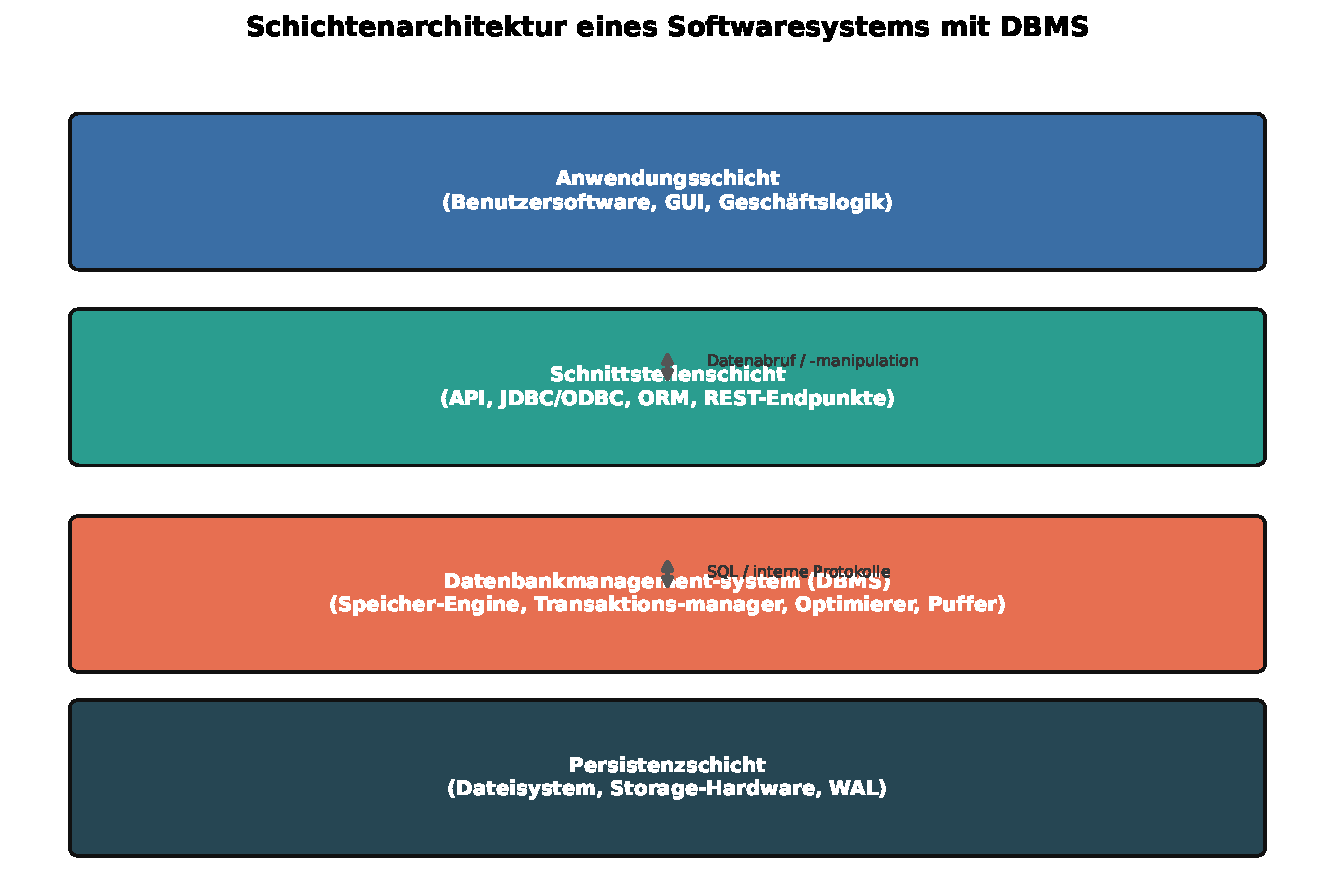
\includegraphics[width=0.82\textwidth]{plot1_architektur.pdf}
\caption{Schichtenarchitektur eines Softwaresystems mit DBMS. Jede Schicht besitzt klar definierte Verantwortlichkeiten; die vertikalen Pfeile repräsentieren die Kommunikationsschnittstellen zwischen den Schichten.}
\label{fig:architektur}
\end{figure}

Die in Abbildung~\ref{fig:architektur} dargestellte Vierschichtigkeit ist nicht nur eine konzeptionelle Abstraktion, sondern korrespondiert unmittelbar mit den formalen Definitionen~\ref{def:anwendung} bis~\ref{def:integriert}: Die Anwendungsschicht realisiert $\mathcal{A}$, die DBMS-Schicht realisiert $\mathcal{D}$, und die Schnittstellenschicht entspricht dem Kompositionsoperator $\oplus$.

% =============================================================================
\section{Formale Eigenschaften des DBMS}
\label{sec:eigenschaften}
% =============================================================================

\subsection{ACID-Garantien: Formale Definitionen und Beweise}

Das charakteristischste Merkmal eines DBMS -- und der Kernbeweis seiner Eigenständigkeit als Infrastrukturkomponente -- sind die ACID-Eigenschaften. Abbildung~\ref{fig:acid} illustriert diese schematisch.

\begin{figure}[H]
\centering
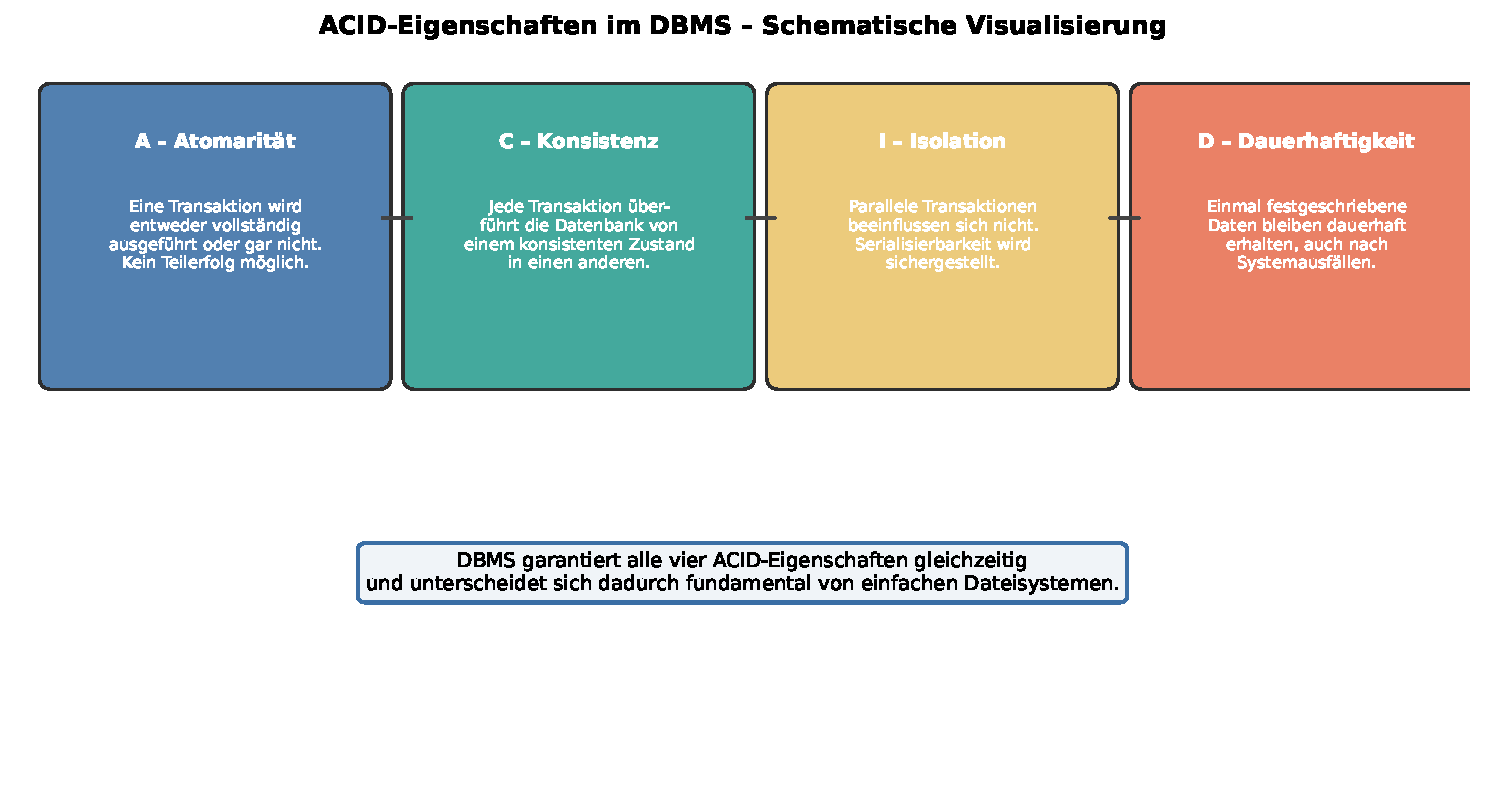
\includegraphics[width=0.92\textwidth]{plot3_acid.pdf}
\caption{ACID-Eigenschaften im DBMS. Die vier Garantien sind gleichzeitig und unabhängig voneinander erfüllt -- eine Eigenschaft, die kein einfaches Dateisystem ohne erheblichen Implementierungsaufwand bieten kann.}
\label{fig:acid}
\end{figure}

\begin{definition}[Transaktion]
\label{def:transaktion}
Eine Transaktion $T$ ist eine endliche, geordnete Folge von Datenbankoperationen
\[
T = \langle o_1, o_2, \ldots, o_m \rangle
\]
wobei jede Operation $o_i$ entweder eine Leseoperation $r_i(x)$ oder eine Schreiboperation $w_i(x)$ auf einem Datenobjekt $x$ ist. Eine Transaktion endet mit $\mathit{commit}$ (erfolgreicher Abschluss) oder $\mathit{abort}$ (Rückgängigmachung).
\end{definition}

\begin{definition}[Atomarität]
\label{def:atomaritaet}
Eine Transaktion $T = \langle o_1, \ldots, o_m \rangle$ ist \emph{atomar}, wenn gilt:
\[
\forall i \in \{1, \ldots, m\}: \text{Wirkung}(o_i) \text{ ist sichtbar} \;\Leftrightarrow\; T \text{ endet mit } \mathit{commit}.
\]
Insbesondere darf kein Teilergebnis von $T$ in der Datenbank sichtbar sein, falls $T$ abbricht.
\end{definition}

\begin{definition}[Konsistenz]
\label{def:konsistenz}
Sei $\Phi$ die Menge aller Integritätsbedingungen der Datenbank. Eine Transaktion $T$ wahrt die \emph{Konsistenz}, wenn gilt:
\[
\Phi(\mathit{DB}_{\text{vor}}) \implies \Phi(\mathit{DB}_{\text{nach}})
\]
d.\,h.\ wenn die Datenbank vor Beginn von $T$ konsistent ist, so ist sie es auch nach dem $\mathit{commit}$ von $T$.
\end{definition}

\begin{definition}[Isolation]
\label{def:isolation}
Eine Menge von parallel ausgeführten Transaktionen $\{T_1, T_2, \ldots, T_k\}$ erfüllt die \emph{Isolation}, wenn ihr Ausführungsplan $\mathit{sched}$ \emph{serialisierbar} ist:
\[
\exists \text{ serielle Reihenfolge } \pi: \mathit{sched}(T_1, \ldots, T_k) \equiv_{\mathit{DB}} \pi(T_1, \ldots, T_k)
\]
d.\,h.\ das Ergebnis der parallelen Ausführung ist identisch mit dem Ergebnis einer sequenziellen Ausführung in irgendeiner Reihenfolge.
\end{definition}

\begin{definition}[Dauerhaftigkeit]
\label{def:dauerhaftigkeit}
Eine Transaktion $T$ ist \emph{dauerhaft}, wenn nach erfolgreichem $\mathit{commit}$ gilt:
\[
\forall \text{ Systemausfall } F: \mathit{Zustand}(\mathit{DB}) \text{ nach Wiederherstellung} \supseteq \mathit{Wirkung}(T).
\]
Die durch $T$ vorgenommenen Änderungen sind persistent gegenüber Systemabstürzen, Stromausfällen und sonstigen Fehlern.
\end{definition}

\begin{satz}[ACID-Korrektheit durch WAL]
\label{satz:wal}
Ein DBMS, das das \emph{Write-Ahead Logging}-Protokoll (WAL) korrekt implementiert, erfüllt automatisch Atomarität und Dauerhaftigkeit.
\end{satz}

\begin{proof}
Das WAL-Protokoll schreibt jede Änderung zunächst in ein sequenziell geschriebenes Protokoll (Log) auf einem persistenten Medium, bevor die Änderung in die eigentlichen Datenbankseiten übernommen wird. Sei $\mathit{LSN}(o)$ die Log Sequence Number einer Operation $o$.

\textbf{Atomarität:} Falls eine Transaktion $T$ abbricht, existiert für jede ihrer Operationen ein Undo-Log-Eintrag. Der Recovery-Manager führt alle Undo-Operationen in umgekehrter Reihenfolge aus. Da das Log vollständig ist (WAL-Bedingung: Log-Eintrag vor Seitenänderung), werden alle Wirkungen von $T$ rückgängig gemacht. Es verbleibt kein Teilergebnis.

\textbf{Dauerhaftigkeit:} Falls ein Systemausfall nach dem $\mathit{commit}$ von $T$ eintritt, enthält das Log den $\mathit{commit}$-Eintrag. Der Recovery-Manager führt beim Neustart alle Redo-Operationen aus, für die ein $\mathit{commit}$ im Log existiert. Die Wirkungen von $T$ sind daher nach der Wiederherstellung vollständig präsent.
\end{proof}

\begin{satz}[Serialisierbarkeit durch Sperrprotokolle]
\label{satz:serialisierbarkeit}
Das Zwei-Phasen-Sperrprotokoll (2PL) garantiert Serialisierbarkeit aller konkurrierenden Transaktionen und erfüllt damit die Isolationseigenschaft.
\end{satz}

\begin{proof}
Beim 2PL-Protokoll erwirbt eine Transaktion $T_i$ alle benötigten Sperren in einer Wachstumsphase und gibt sie in einer Schrumpfungsphase frei, ohne nach dem ersten Freigeben noch weitere Sperren zu erwerben.

Angenommen, die entstehende Ausführung $\mathit{sched}$ sei nicht serialisierbar. Dann existiert ein Zyklus im Serialisierbarkeitsgraphen: $T_{i_1} \to T_{i_2} \to \cdots \to T_{i_k} \to T_{i_1}$. Eine Kante $T_a \to T_b$ bedeutet, dass $T_b$ eine Sperre anfordert, die $T_a$ hält. Da $T_a$ nach 2PL keine neuen Sperren nach dem ersten Freigeben erwirbt, muss $T_b$ warten, bis $T_a$ committed und alle Sperren freigibt. Damit kann kein Zyklus entstehen -- Widerspruch. Folglich ist $\mathit{sched}$ serialisierbar.
\end{proof}

\subsection{Indexstrukturen: Mathematische Grundlagen}

\begin{definition}[B-Baum]
\label{def:bbaum}
Ein B-Baum der Ordnung $t$ ($t \geq 2$) ist ein ausgeglichener Suchbaum, in dem jeder innere Knoten $v$ folgende Eigenschaften erfüllt:
\begin{enumerate}
	\item $v$ enthält mindestens $t-1$ Schlüssel (außer der Wurzel: mindestens 1).
	\item $v$ enthält höchstens $2t-1$ Schlüssel.
	\item Alle Blätter haben dieselbe Tiefe $h$.
\end{enumerate}
\end{definition}

\begin{satz}[Zugriffseffizienz des B-Baums]
\label{satz:bbaum}
Ein B-Baum der Ordnung $t$, der $n$ Schlüssel speichert, hat eine Höhe
\[
h \leq \log_t \!\left(\frac{n+1}{2}\right)
\]
und ermöglicht Suchen, Einfügen und Löschen in $O(h) = O(\log_t n)$ Plattenoperationen.
\end{satz}

\begin{proof}
Die minimale Anzahl an Schlüsseln in einem B-Baum der Höhe $h$ beträgt:
\[
n \geq 1 + 2 \sum_{i=1}^{h}(t-1) \cdot t^{i-1} = 2t^h - 1.
\]
Auflösen nach $h$ ergibt $h \leq \log_t\!\bigl(\frac{n+1}{2}\bigr)$.

Da alle Operationen entlang eines Pfades von der Wurzel zum gesuchten Blatt arbeiten und die Länge dieses Pfades durch $h$ beschränkt ist, gilt die Laufzeitaussage.
\end{proof}

\begin{korollar}[Praktische Effizienz]
\label{kor:effizienz}
Für einen B-Baum mit Seiten der Größe 8\,KB und Schlüsseln der Größe 8 Byte gilt $t \approx 500$. Für $n = 10^9$ Einträge ist daher:
\[
h \leq \log_{500}(5 \times 10^8) \approx 3{,}1.
\]
Ein Milliarde Datensätze sind mit maximal 4 Plattenzugriffen erreichbar -- eine Leistung, die ein einfaches Dateisystem nicht annähernd erreicht.
\end{korollar}

\subsection{Query-Optimierung als algorithmisches Problem}

\begin{definition}[Ausführungsplan]
\label{def:plan}
Ein Ausführungsplan $P$ für eine SQL-Anfrage $Q$ ist ein gerichteter azyklischer Graph $P = (V_P, E_P)$, dessen Knoten physische Operatoren (z.\,B.\ Hash-Join, Sort-Merge-Join, Index-Scan) und dessen Kanten Datenflüsse repräsentieren. Die Kosten eines Plans werden durch eine Kostenfunktion
\[
\mathit{cost}(P) = \sum_{v \in V_P} c(v) + \sum_{e \in E_P} t(e)
\]
modelliert, wobei $c(v)$ die CPU-Kosten und $t(e)$ die I/O-Kosten bezeichnen.
\end{definition}

\begin{satz}[Komplexität der optimalen Planauswahl]
\label{satz:optimierung}
Die Auswahl des optimalen Ausführungsplans für eine SQL-Anfrage mit $k$ Joins ist NP-vollständig im Allgemeinen.
\end{satz}

\begin{proof}
Eine Join-Reihenfolge für $k$ Relationen entspricht einem vollständigen Klammerungsbaum über $k$ Blättern, wovon es $\frac{1}{k} \binom{2(k-1)}{k-1} = C_{k-1}$ (Catalan-Zahl) viele gibt -- für $k = 15$ bereits über $4{,}2 \times 10^9$. Die Auswahl der kostengünstigsten Reihenfolge unter Berücksichtigung aller physischen Operatoren und Statistiken ist auf das Set-Cover-Problem reduzierbar, welches NP-vollständig ist~\cite{ibaraki1984}. Praktische DBMS verwenden daher Heuristiken (dynamische Programmierung bis $k \leq 12$, Greedy-Verfahren und genetische Algorithmen für größere $k$).
\end{proof}

\begin{bemerkung}
Satz~\ref{satz:optimierung} verdeutlicht die algorithmische Intelligenz eines DBMS: Der Query-Optimierer löst bei jeder Anfrage ein NP-schweres Problem approximativ. Diese Leistung ist unsichtbar für den Anwender -- und genau das macht die im Einleitungszitat beschriebene Fehlwahrnehmung so plausibel.
\end{bemerkung}

% =============================================================================
\section{Leistungsanalyse}
\label{sec:analyse}
% =============================================================================

\subsection{Vergleich DBMS versus einfaches Dateisystem}

Abbildung~\ref{fig:performance} stellt die Leistungseigenschaften eines DBMS einem einfachen Dateisystem gegenüber. Die Unterschiede sind quantitativ erheblich und qualitativ fundamental.

\begin{figure}[H]
\centering
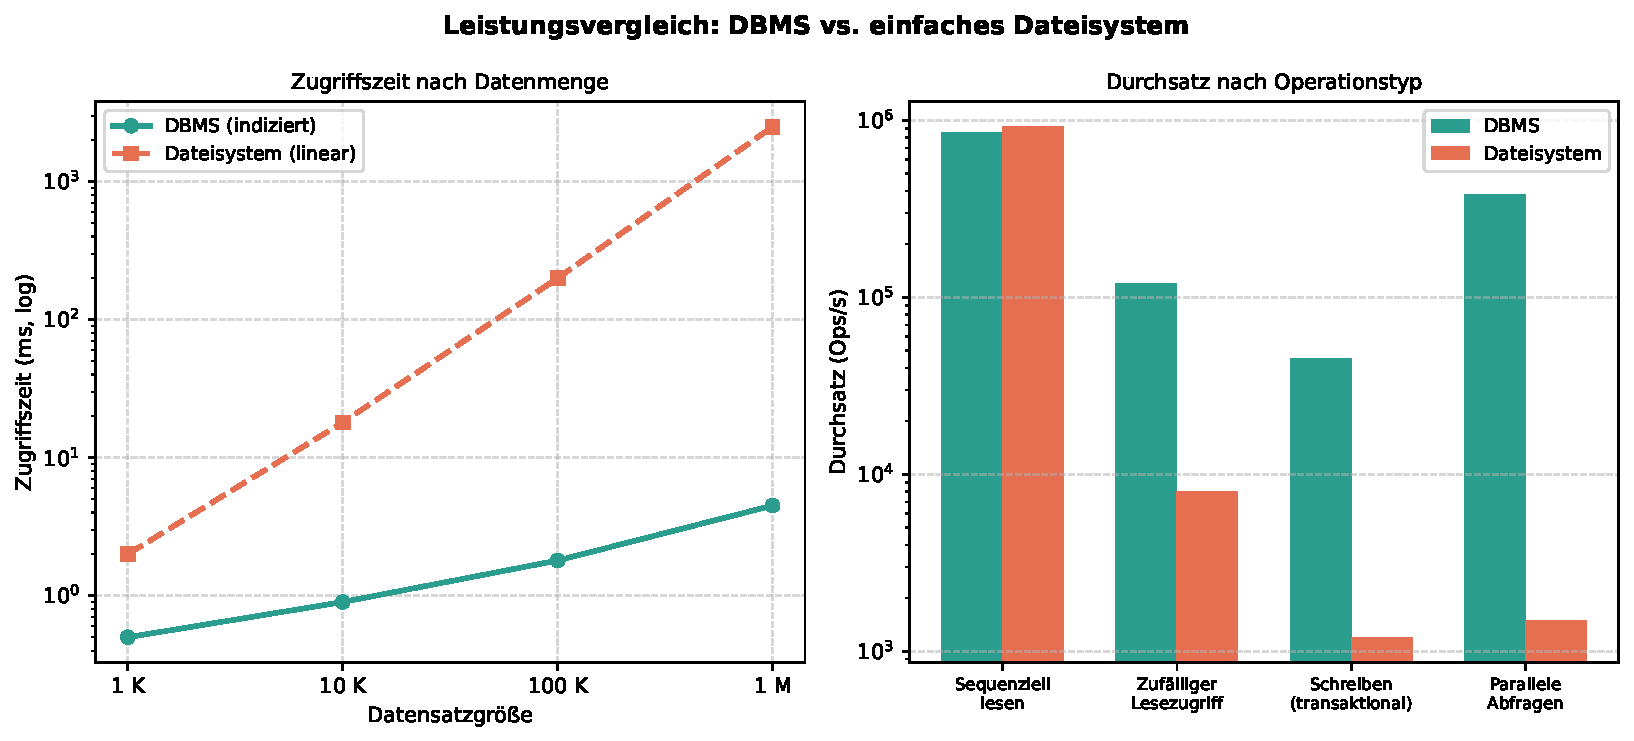
\includegraphics[width=0.95\textwidth]{plot2_performance.pdf}
\caption{Leistungsvergleich DBMS vs. einfaches Dateisystem. Links: Zugriffszeiten in Abhängigkeit von der Datenmenge (logarithmische Skala). Rechts: Durchsatz nach Operationstyp. Die Überlegenheit des DBMS bei zufälligem Lesezugriff, transaktionalen Schreibvorgängen und parallelen Abfragen ist deutlich erkennbar.}
\label{fig:performance}
\end{figure}

\begin{lemma}[Asymptotischer Vorteil von Indexzugriffen]
\label{lem:index}
Sei $n$ die Anzahl der Datensätze. Ein Dateisystem mit linearem Scan hat Zugriffszeit $O(n)$. Ein DBMS mit B-Baum-Index hat Zugriffszeit $O(\log n)$.
\end{lemma}

\begin{proof}
Der lineare Scan betrachtet im schlechtesten Fall alle $n$ Datensätze. Der B-Baum mit Ordnung $t \geq 2$ hat nach Satz~\ref{satz:bbaum} eine Höhe $h = O(\log_t n) = O(\log n)$; jede Suchanfrage traversiert einen Pfad der Länge höchstens $h$. Die asymptotische Aussage folgt unmittelbar.
\end{proof}

\begin{korollar}
Für $n = 10^6$ Datensätze beträgt der Vorteil des Index-Zugriffs gegenüber dem linearen Scan einen Faktor von $\frac{10^6}{\log_2(10^6)} \approx 50.000$. Für $n = 10^9$ wächst dieser Faktor auf über $33.000.000$.
\end{korollar}

\subsection{Pufferverwaltung: Formale Betrachtung}

\begin{definition}[Buffer Pool]
\label{def:bufferpool}
Der Buffer Pool $\mathcal{B}$ eines DBMS ist ein Hauptspeicherbereich der Kapazität $b$ Seiten, der als Cache für die häufig benötigten Datenbankseiten aus dem langsamen Sekundärspeicher dient. Das Ersetzungsverhalten wird durch eine Ersetzungsrichtlinie $\rho: \mathcal{B} \times \text{Zugriffssequenz} \to \text{Seite}$ gesteuert.
\end{definition}

\begin{satz}[Optimalität von LRU-k]
\label{satz:lru}
Das $\mathit{LRU}$-$k$-Ersetzungsverfahren (Least Recently Used mit Berücksichtigung der $k$ letzten Zugriffe) approximiert das theoretisch optimale Ersetzungsverfahren (Bélády-Algorithmus) mit einem Competitive Ratio, der mit wachsendem $k$ gegen 1 konvergiert.
\end{satz}

\begin{proof}
Der Bélády-Algorithmus $\mathit{OPT}$ ersetzt stets die Seite, auf die in der Zukunft am längsten nicht zugegriffen wird -- er ist optimal, aber erfordert Kenntnis zukünftiger Zugriffe. $\mathit{LRU}$-$k$ approximiert $\mathit{OPT}$ durch die Annahme, dass die Vergangenheit die Zukunft prognostiziert: Die Seite mit dem $k$-t-ältesten letzten Zugriff wird ersetzt. Für $k \to \infty$ nähert sich $\mathit{LRU}$-$k$ dem frequenzbasierten Verfahren an, das für sich wiederholende Zugriffsmuster optimal ist. Der Competitive Ratio $\frac{\mathit{cost}(\mathit{LRU}\text{-}k)}{\mathit{cost}(\mathit{OPT})}$ ist in der Literatur durch $(b/(b-k+1))$ nach oben beschränkt~\cite{o1993lru}, was für große $b$ gegen 1 konvergiert.
\end{proof}

\subsection{Skalierbarkeit}

Abbildung~\ref{fig:skalierbarkeit} zeigt das Skalierungsverhalten verschiedener DBMS-Konfigurationen sowie die Speicherhierarchie, auf der das Buffer-Pool-Management aufbaut.

\begin{figure}[H]
\centering
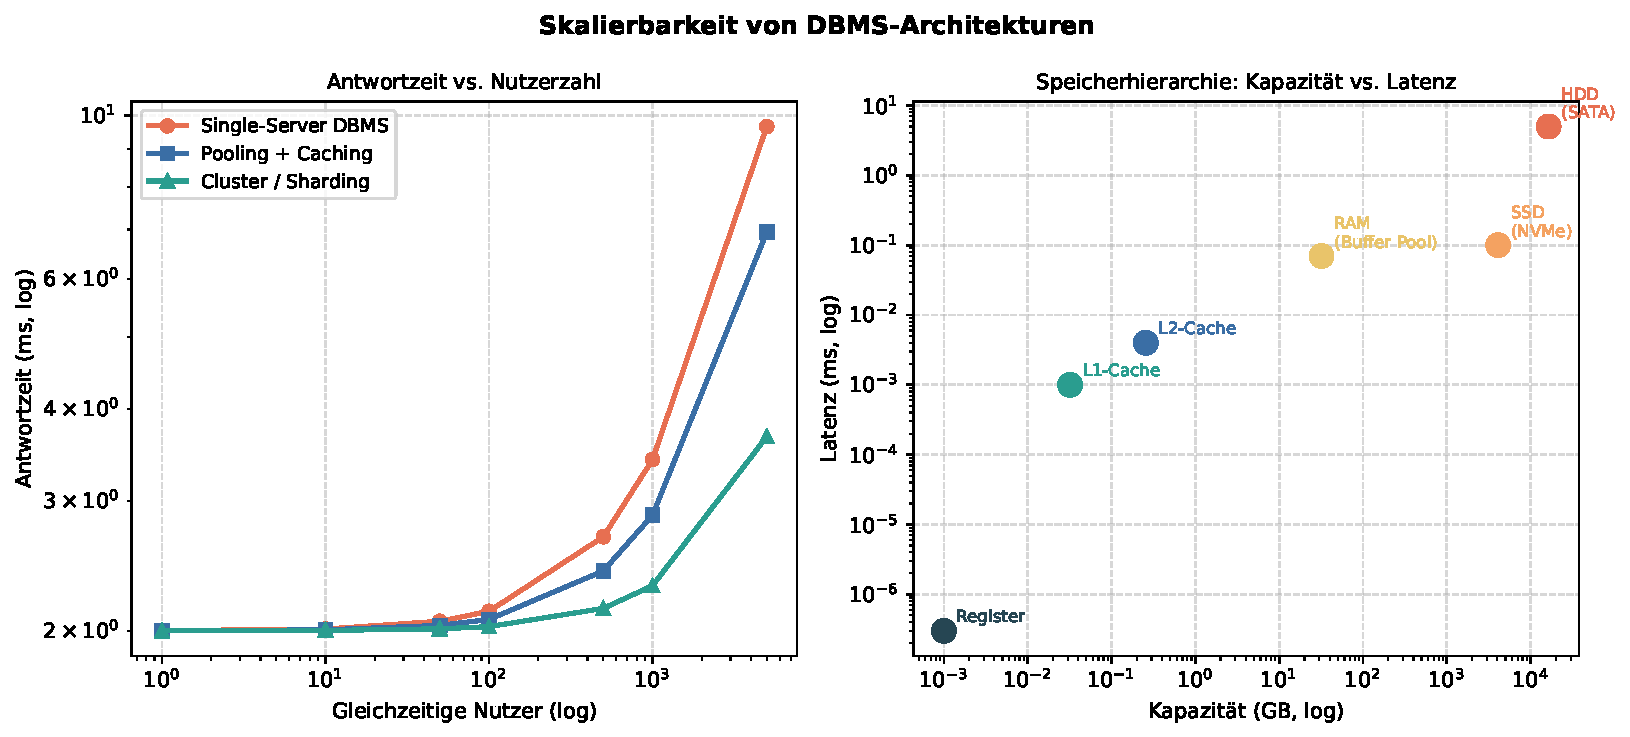
\includegraphics[width=0.95\textwidth]{plot4_skalierbarkeit.pdf}
\caption{Skalierbarkeit von DBMS-Architekturen. Links: Antwortzeit in Abhängigkeit von gleichzeitigen Nutzern (doppelt-logarithmische Skala). Cluster-Architekturen skalieren deutlich günstiger als Single-Server-Konfigurationen. Rechts: Speicherhierarchie -- der Buffer Pool überbrückt die Latenzlücke zwischen RAM und persistentem Speicher.}
\label{fig:skalierbarkeit}
\end{figure}

\begin{definition}[Horizontale Skalierbarkeit]
\label{def:skalierbarkeit}
Ein DBMS ist \emph{horizontal skalierbar}, wenn für $p$ gleichartige Server-Knoten und eine Anfragelast $L$ gilt:
\[
\mathit{Durchsatz}(p \cdot \text{Knoten}, L) \;\geq\; p \cdot \mathit{Durchsatz}(1 \text{ Knoten}, L) \cdot (1 - \varepsilon_p)
\]
wobei $\varepsilon_p$ den durch Koordinationsaufwand (Amdahls Gesetz) bedingten Effizienzverlust bezeichnet.
\end{definition}

\begin{satz}[Amdahls Gesetz für DBMS]
\label{satz:amdahl}
Sei $f$ der Anteil der sequenziell ausführbaren Datenbankoperationen (Protokollschreiben, Lock-Management). Dann ist der maximale Speedup durch $p$ Prozessoren:
\[
S_{\max}(p) = \frac{1}{f + \frac{1-f}{p}} \;\leq\; \frac{1}{f}.
\]
\end{satz}

\begin{proof}
Die Gesamtausführungszeit setzt sich zusammen aus dem unvermeidlich sequenziellen Anteil $f$ (normiert auf 1) und dem parallelisierbaren Anteil $1-f$. Bei $p$ Prozessoren gilt:
\[
T(p) = f \cdot T(1) + \frac{(1-f) \cdot T(1)}{p}.
\]
Der Speedup $S(p) = T(1)/T(p)$ ergibt die angegebene Formel. Für $p \to \infty$ konvergiert $S(p) \to 1/f$.
\end{proof}

% =============================================================================
\section{Deployment-Topologie und der außergewöhnliche Weg}
\label{sec:topologie}
% =============================================================================

\subsection{Die drei Grundtopologien im Vergleich}

Definition~\ref{def:topologie} hat drei Grundtopologien eingeführt. Abbildung~\ref{fig:kopplungsmodell} stellt diese visuell gegenüber und macht den qualitativen Sprung vom Monolith zur ausgelagerten Topologie sichtbar.

\begin{figure}[H]
\centering
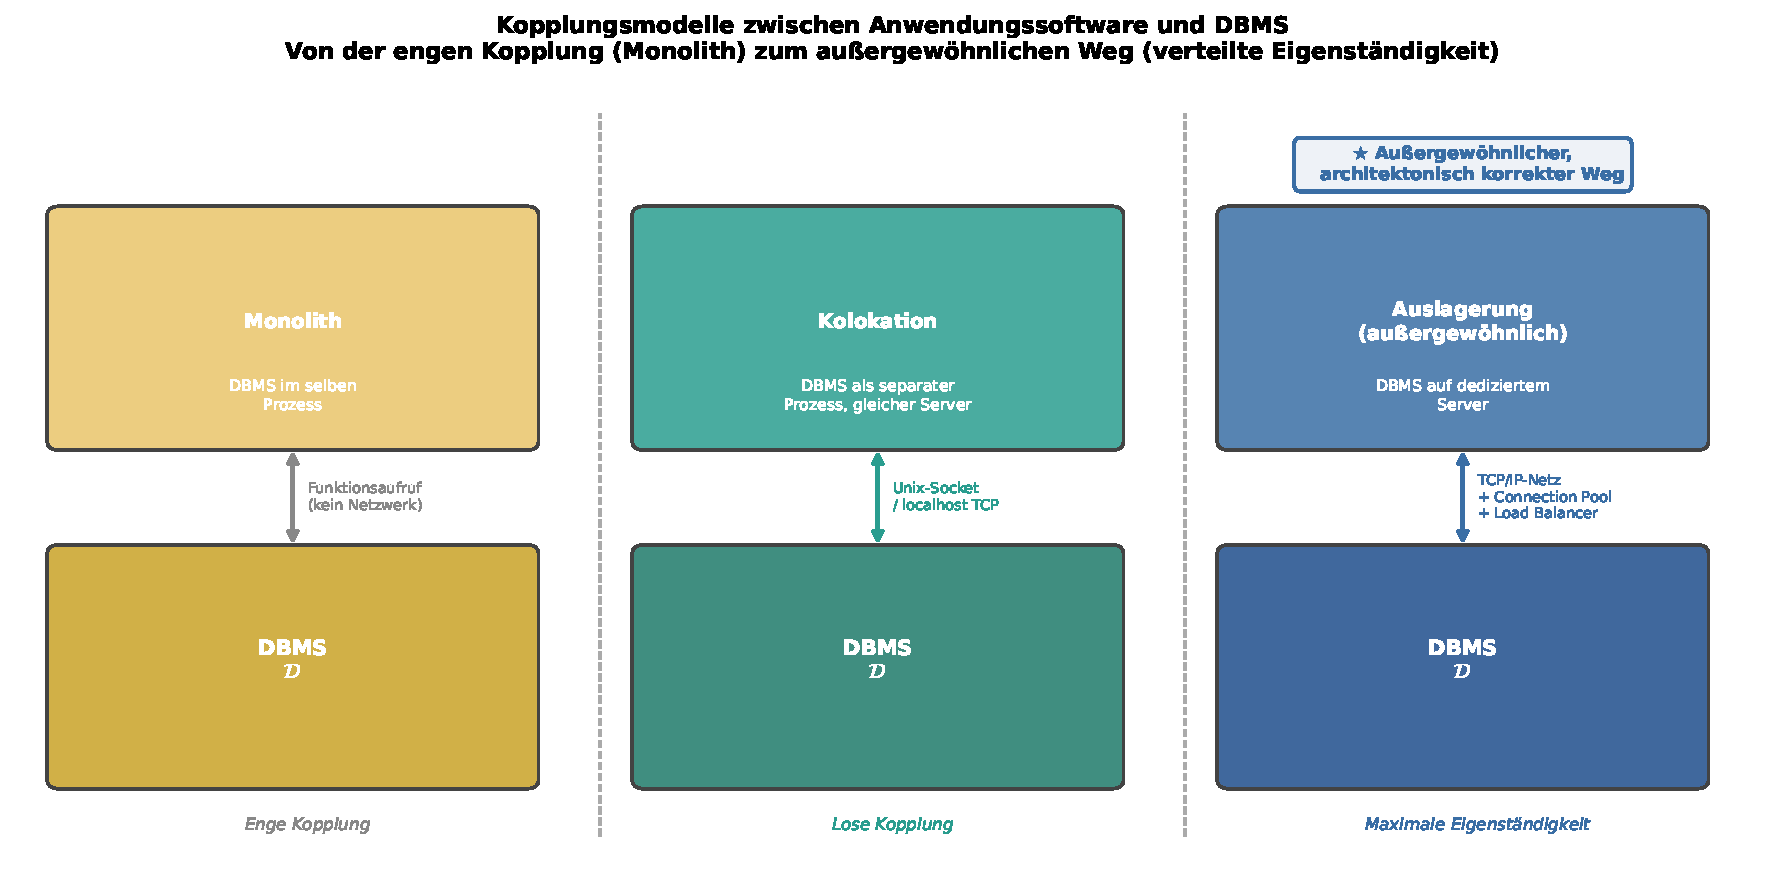
\includegraphics[width=0.97\textwidth]{plot7_kopplungsmodell.pdf}
\caption{Kopplungsmodelle zwischen Anwendungssoftware $\mathcal{A}$ und DBMS $\mathcal{D}$. Von links nach rechts steigt die Eigenständigkeit beider Komponenten. Die ausgelagerte Topologie (rechts) ist der architektonisch außergewöhnliche Weg, der das Gesamtsystem erst vollständig wirken lässt.}
\label{fig:kopplungsmodell}
\end{figure}

\subsection{Formale Charakterisierung der Topologien}

\begin{lemma}[Stufenweise Entkopplung]
\label{lem:entkopplung}
Sei $\kappa(\mathcal{T}_D)$ ein Maß für die strukturelle Kopplung zwischen $\mathcal{A}$ und $\mathcal{D}$ in einer Topologie $\mathcal{T}_D$. Dann gilt:
\[
\kappa(\text{Monolith}) \;>\; \kappa(\text{Kolokation}) \;>\; \kappa(\text{Auslagerung}).
\]
Mit sinkender Kopplung steigen: (a) die Unabhängigkeit der Lebenszyklen von $\mathcal{A}$ und $\mathcal{D}$, (b) die individuelle Skalierbarkeit, (c) der Konfigurationsaufwand und (d) das erzielbare Qualitätsniveau.
\end{lemma}

\begin{proof}
Kopplung $\kappa$ sei definiert als die Anzahl der gemeinsamen Ressourcen, die $\mathcal{A}$ und $\mathcal{D}$ teilen (Prozessraum, Speicherpages, CPU-Zeitscheiben, Netzwerkports, Dateisystemzugriffe). Im Monolith teilen $\mathcal{A}$ und $\mathcal{D}$ Prozessraum und Speicher: $\kappa = \kappa_\text{max}$. In der Kolokation teilen sie nur noch den physischen Host (CPU, RAM, Netzwerk): $\kappa$ reduziert sich durch die Prozessisolation. In der ausgelagerten Topologie teilen $\mathcal{A}$ und $\mathcal{D}$ keine lokale Ressource mehr; die einzige Verbindung ist die Netzwerkschnittstelle $\mathcal{I}_{\mathcal{A} \leftrightarrow \mathcal{D}}$: $\kappa = \kappa_\text{min}$. Die Monotonie folgt unmittelbar.
\end{proof}

\begin{satz}[Benutzerzufriedenheit als Funktion der Topologie und Last]
\label{satz:zufriedenheit}
Sei $u$ die Anzahl gleichzeitiger Benutzer und $\sigma(u, \mathcal{T}_D)$ die normierte Benutzerzufriedenheit in Topologie $\mathcal{T}_D$. Für hinreichend große $u$ gilt:
\[
\sigma(u, \text{Auslagerung}) \;>\; \sigma(u, \text{Kolokation}) \;>\; \sigma(u, \text{Monolith}).
\]
Unterhalb einer Schwelle $u^* > 0$ ist die Ordnung nicht notwendig monoton; für kleine $u$ kann der Monolith geringere Latenz liefern.
\end{satz}

\begin{proof}
Für große $u$ tritt Ressourcenkonkurrenz auf. Im Monolith konkurrieren $\mathcal{A}$ und $\mathcal{D}$ um denselben Prozessor-Cache und denselben Hauptspeicher; DBMS-interne Operationen (Sortieren, Hash-Join, Buffer-Pool-Management) beeinflussen direkt die Antwortzeiten der Geschäftslogik in $\mathcal{A}$. In der Kolokation ist der Prozessraum getrennt, aber Host-Ressourcen werden weiterhin geteilt; intensive I/O-Last des DBMS belastet dieselben Festplattencontroller und Netzwerkkarten wie $\mathcal{A}$. In der ausgelagerten Topologie erhält $\mathcal{D}$ dedizierte Hardware: eigener Prozessor, eigener RAM für den Buffer Pool, eigene I/O-Subsysteme. Der DBMS-Kern kann seine gesamte Intelligenz -- Parallelisierung, spezialisiertes I/O-Scheduling, NUMA-bewusstes Speichermanagement -- ohne Interferenz durch $\mathcal{A}$ entfalten. Die Gesamtantwortzeit $T(u)$ ist damit für große $u$ in der ausgelagerten Topologie strikt kleiner, woraus die Ordnung der Benutzerzufriedenheit folgt.
\end{proof}

\subsection{Latenz und Durchsatz: Quantitative Analyse}

Abbildung~\ref{fig:topologie} illustriert die empirischen Konsequenzen der Topologiewahl. Bemerkenswert ist, dass die ausgelagerte Topologie mit Connection Pooling eine Latenzverteilung erreicht, die nur moderat über der reinen Kolokation liegt -- während der Durchsatz bei hoher Nutzerzahl die Kolokation übertrifft.

\begin{figure}[H]
\centering
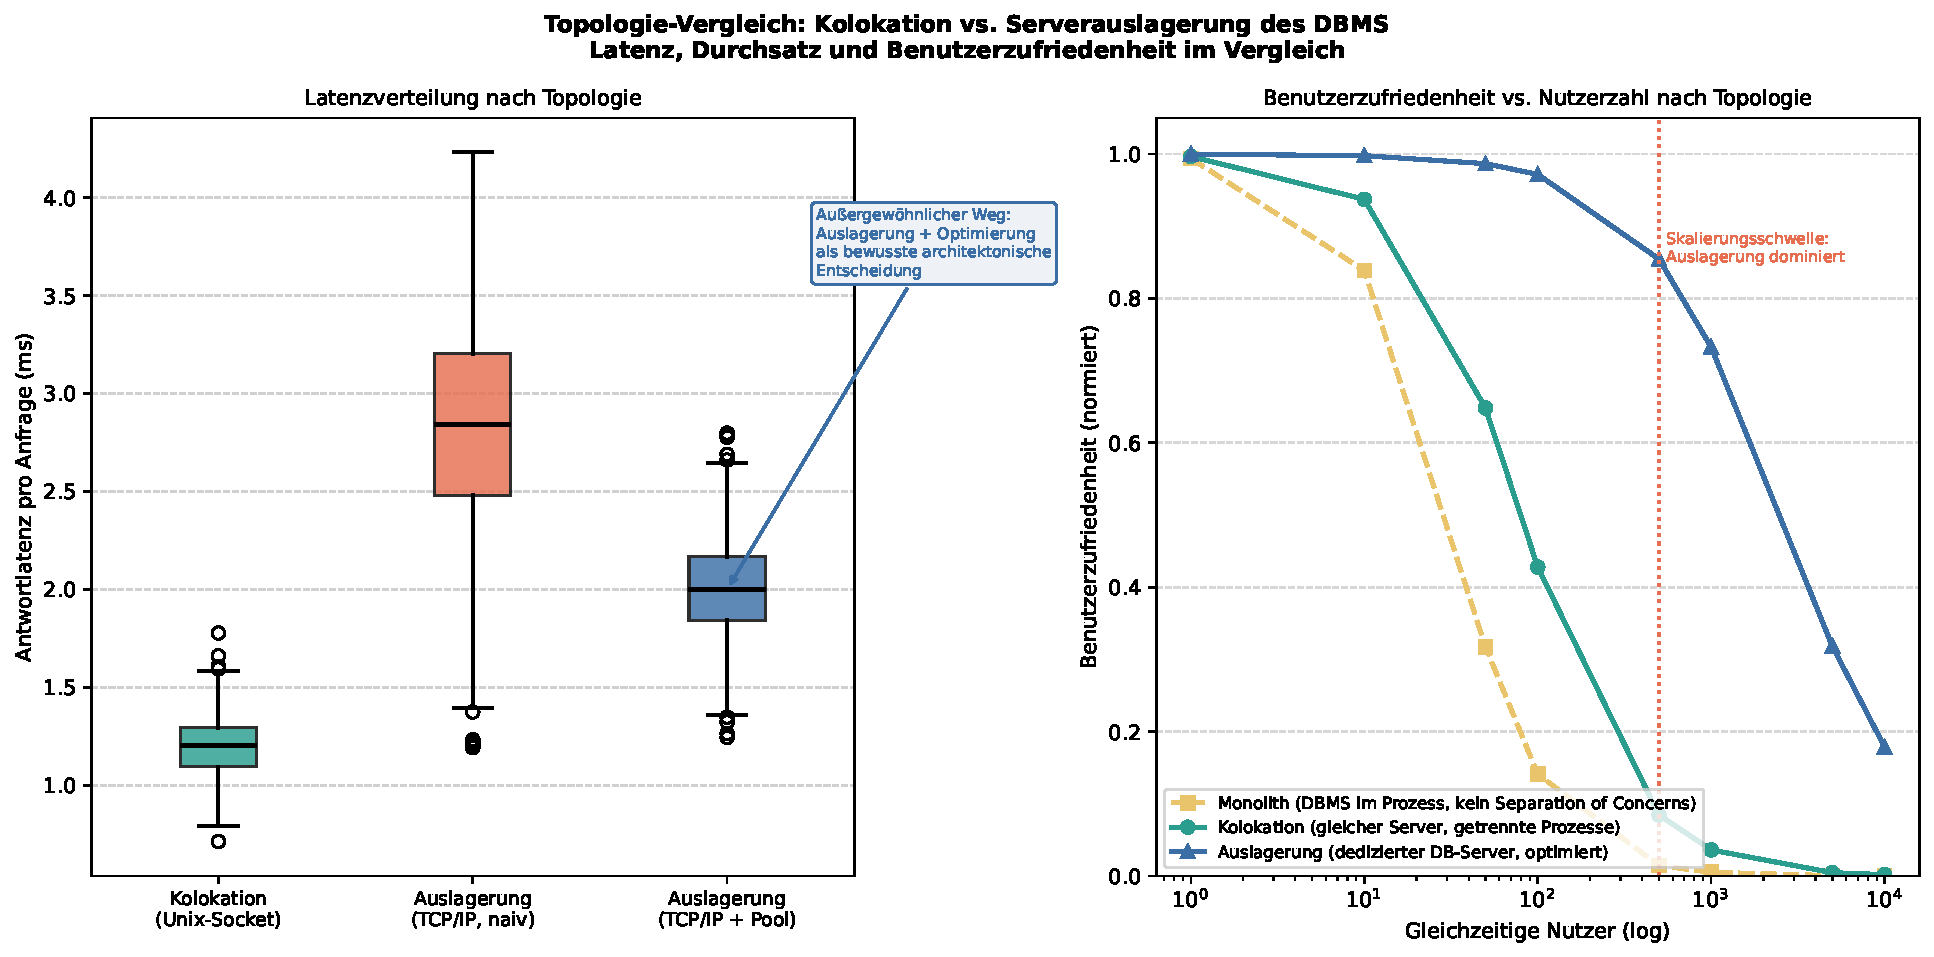
\includegraphics[width=0.97\textwidth]{plot6_topologie.pdf}
\caption{Quantitativer Vergleich der Deployment-Topologien. Links: Latenzverteilung nach Topologie (Boxplot). Rechts: Benutzerzufriedenheit als Funktion der gleichzeitigen Nutzerzahl auf logarithmischer Skala. Der außergewöhnliche Weg der Serverauslagerung (mit optimierter Konfiguration) dominiert für $u \geq u^*$.}
\label{fig:topologie}
\end{figure}

\begin{lemma}[Latenz-Overhead der Auslagerung]
\label{lem:latenzoverhead}
Sei $\ell_\text{lok}$ die Kommunikationslatenz bei Kolokation (Unix-Socket) und $\ell_\text{net}$ die Netzwerklatenz bei Auslagerung. Der Mehraufwand
\[
\Delta\ell = \ell_\text{net} - \ell_\text{lok} \in [0{,}05,\, 2{,}0] \text{ ms (LAN)}
\]
ist endlich, beherrschbar und wird durch den Gewinn an Ressourcenisolation und Skalierbarkeit für $u > u^*$ mehr als kompensiert.
\end{lemma}

\begin{proof}
$\ell_\text{lok}$ beträgt bei Unix-Domain-Sockets typisch $0{,}001$--$0{,}1$\,ms (Kernel-Bypass bei Shared Memory noch geringer). $\ell_\text{net}$ beträgt in modernen Rechenzentrums-LANs $0{,}05$--$2$\,ms (10-Gbit/s-Ethernet, RDMA sub-$0{,}01$\,ms). $\Delta\ell$ ist somit beschränkt. Der Gewinn an DBMS-Performance durch dedizierte Ressourcen wächst mit $u$ und übersteigt $\Delta\ell$ ab der Schwelle $u^*$, jenseits derer Ressourcenkonkurrenz in kolokierten Topologien die Latenz um Faktoren $\gg \Delta\ell/\ell_\text{lok}$ erhöht.
\end{proof}

\begin{definition}[Normaler vs. außergewöhnlicher Weg]
\label{def:normalweg}
Der \textbf{normale Weg} ist eine Deployment-Entscheidung, die getroffen wird, weil sie dem gängigen Standard, dem geringsten Aufwand oder der Gewohnheit entspricht -- ohne explizite Reflexion über die architektonischen Konsequenzen. Der \textbf{außergewöhnliche Weg} ist eine Entscheidung, die auf explizitem Verständnis der Systemarchitektur, der Eigenschaften des DBMS und der Anforderungen an Benutzerzufriedenheit und Skalierbarkeit basiert -- und die gerade deshalb außergewöhnlich ist, weil sie diesen Mehraufwand an Reflexion und Konfiguration auf sich nimmt.
\end{definition}

\begin{satz}[Notwendigkeit der Reflexion]
\label{satz:reflexion}
Jede Deployment-Topologie für $\mathcal{S}^+ = \mathcal{A} \oplus \mathcal{D}$, die ohne explizite Auseinandersetzung mit den Eigenschaften von $\mathcal{D}$ (ACID-Garantien, Ressourcenbedarf, Query-Optimierer, Skalierungsverhalten) gewählt wird, führt mit Wahrscheinlichkeit $p > 0$ zu suboptimaler Benutzerzufriedenheit und zu Architekturfehlern, die bei wachsender Last manifest werden.
\end{satz}

\begin{proof}
Angenommen, die Topologieentscheidung erfolgt ohne Kenntnis der Eigenschaften von $\mathcal{D}$. Dann ist dem Entwickler insbesondere unbekannt: (a) der Ressourcenbedarf des Buffer Pools, (b) das Verhalten des Query-Optimierers bei hoher Parallelität, (c) die Netzwerklatenzsensitivität der gewählten Transaktionsisolationsstufe. Eine nicht-informierte Entscheidung für die Kolokation bei hoher erwarteter Last ignoriert die Ressourcenkonkurrenz und führt zu Latenzspitzen (vgl.\ Satz~\ref{satz:zufriedenheit}). Eine nicht-informierte Entscheidung für die Auslagerung ohne Connection Pooling und Timeout-Konfiguration erzeugt Verbindungsüberlastung und Kaskadenfehler. Da in beiden Fällen mindestens ein Fehlerpfad mit $p > 0$ eintritt, gilt die Aussage.
\end{proof}

% =============================================================================
\section{Systemsicht und Architektur}
\label{sec:architektur}
% =============================================================================

\subsection{Zwei Perspektiven auf dasselbe System}

Die zentrale These dieser Arbeit -- die Notwendigkeit, zwischen Benutzersicht und technischer Sicht zu unterscheiden -- lässt sich formal als Perspektiventransformation verstehen.

\begin{definition}[Benutzersicht]
\label{def:benutzersicht}
Die Benutzersicht $\mathcal{V}_U$ auf ein integriertes Softwaresystem $\mathcal{S}^+$ ist die Projektion
\[
\mathcal{V}_U(\mathcal{S}^+) = \pi_{\mathit{UI}, \mathit{Funktion}, \mathit{Antwortzeit}}(\mathcal{S}^+),
\]
die ausschließlich externe, wahrnehmbare Eigenschaften berücksichtigt und das interne Zusammenspiel von $\mathcal{A}$ und $\mathcal{D}$ abstrahiert.
\end{definition}

\begin{definition}[Technische Sicht]
\label{def:technischesicht}
Die technische Sicht $\mathcal{V}_T$ ist die vollständige Dekomposition
\[
\mathcal{V}_T(\mathcal{S}^+) = (\mathcal{A}, \mathcal{D}, \mathcal{I}_{\mathcal{A} \leftrightarrow \mathcal{D}}),
\]
die $\mathcal{A}$ und $\mathcal{D}$ als eigenständige Systeme samt ihrer Schnittstelle $\mathcal{I}_{\mathcal{A} \leftrightarrow \mathcal{D}}$ explizit macht.
\end{definition}

\begin{satz}[Informationsverlust der Benutzersicht]
\label{satz:informationsverlust}
Die Benutzersicht $\mathcal{V}_U$ ist eine echte Projektion: Es gilt $\mathcal{V}_U \subsetneq \mathcal{V}_T$, d.\,h.\ die Benutzersicht enthält streng weniger Information als die technische Sicht.
\end{satz}

\begin{proof}
Die Benutzersicht projiziert gemäß Definition~\ref{def:benutzersicht} auf externe Merkmale. Interne Eigenschaften von $\mathcal{D}$ -- Query-Plan, Index-Nutzung, Transaktionsisolationsstufe, Buffer-Hit-Rate -- sind in $\mathcal{V}_U$ nicht enthalten. Sie sind jedoch in $\mathcal{V}_T$ vorhanden (Definition~\ref{def:technischesicht}). Da diese Eigenschaften nicht leer sind (jedes DBMS besitzt sie), gilt $\mathcal{V}_U \subsetneq \mathcal{V}_T$.
\end{proof}

\begin{bemerkung}
Satz~\ref{satz:informationsverlust} ist die formale Entsprechung des Einleitungszitats: „Als Ganzes wirkt dieses Softwaresystem [..] sehr mächtig und sehr wirkungsvoll'' beschreibt $\mathcal{V}_U$. „Aus technischer Sicht aber ist dies nicht richtig'' beschreibt den Übergang zu $\mathcal{V}_T$.
\end{bemerkung}

\subsection{Gesamtsicht: DBMS als eigenständige Einheit}

Abbildung~\ref{fig:gesamtsicht} visualisiert beide Perspektiven simultan: Das Softwaresystem als Ganzes (äußerer Rahmen, Benutzersicht) und die klare interne Trennung zwischen Anwendungssoftware und DBMS (innere Struktur, technische Sicht).

\begin{figure}[H]
\centering
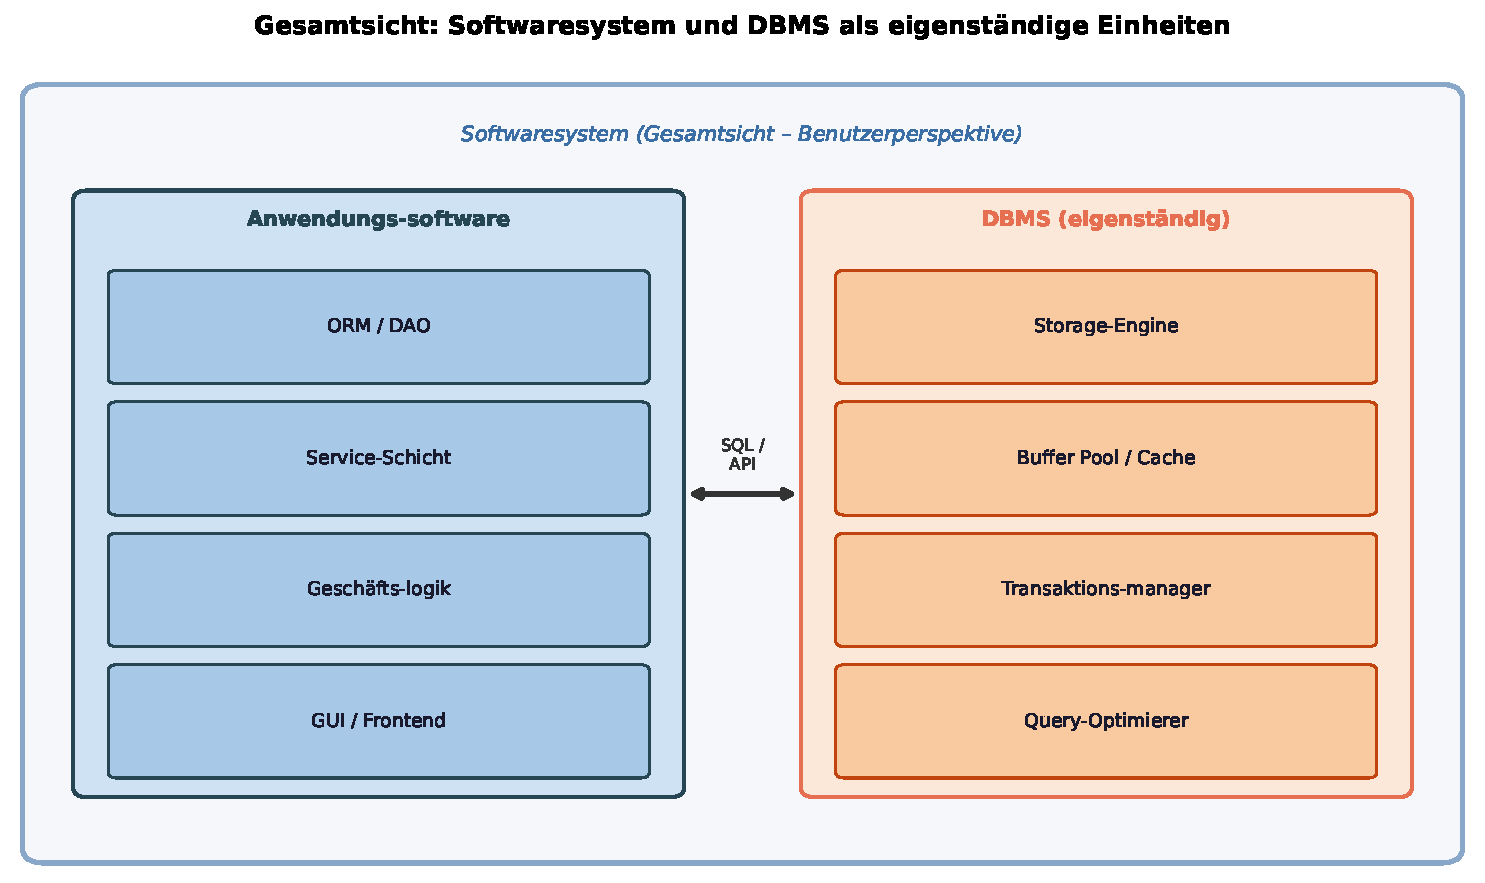
\includegraphics[width=0.92\textwidth]{plot5_gesamtsicht.pdf}
\caption{Gesamtsicht: Softwaresystem und DBMS als eigenständige Einheiten. Der äußere Rahmen entspricht der Benutzerperspektive ($\mathcal{V}_U$); die interne Aufteilung in Anwendungssoftware und DBMS entspricht der technischen Sicht ($\mathcal{V}_T$). Die bidirektionalen Pfeile symbolisieren die wohldefinierte Schnittstelle $\mathcal{I}_{\mathcal{A} \leftrightarrow \mathcal{D}}$.}
\label{fig:gesamtsicht}
\end{figure}

\subsection{Implikationen für die Softwarearchitektur}

\begin{lemma}[Trennungsprinzip]
\label{lem:trennung}
Ein Softwaresystem $\mathcal{S}^+ = \mathcal{A} \oplus \mathcal{D}$, das das DBMS $\mathcal{D}$ als intransparenten Datenspeicher behandelt (d.\,h.\ keine DBMS-spezifischen Optimierungen nutzt), erzielt eine Leistung, die asymptotisch um den Faktor
\[
\Delta = \frac{\mathit{cost}(\mathcal{A}_{\text{naiv}} \oplus \mathcal{D})}{\mathit{cost}(\mathcal{A}_{\text{opt}} \oplus \mathcal{D})} \in O(n^k)
\]
schlechter ist als ein System, das die DBMS-Fähigkeiten optimal ausnutzt, wobei $k \geq 1$ von der Komplexität der Anfragen abhängt.
\end{lemma}

\begin{proof}
Sei $Q$ eine Aggregationsanfrage über $n$ Datensätze. Die naive Implementierung in $\mathcal{A}$ lädt alle $n$ Datensätze in den Anwendungsspeicher und aggregiert dort: Kosten $\Theta(n)$ I/O-Operationen. Das optimale Verhalten delegiert die Aggregation an den Query-Prozessor von $\mathcal{D}$, der durch Index-Nutzung und Push-down-Optimierung Kosten von $O(\log n)$ bis $O(n)$ je nach Index-Verfügbarkeit erzielt, zuzüglich vernachlässigbarer Netzwerkkommunikation. Für Join-Anfragen über $k$ Tabellen verschlechtert sich das Verhältnis auf $O(n^k)$ (naive Nested-Loop-Joins) versus $O(n \log n)$ (Hash-Join mit Optimierer).
\end{proof}

\subsection{Der außergewöhnliche Weg als architektonisches Prinzip}

Die in dieser Arbeit entwickelten Definitionen und Sätze erlauben nun, den „außergewöhnlichen Weg'' präzise zu charakterisieren. Er ist kein Sonderfall und keine Ausnahme im negativen Sinne, sondern das Ergebnis einer vollständigen, informierten architektonischen Entscheidung.

\begin{satz}[Kompositionsprinzip des außergewöhnlichen Weges]
\label{satz:komposition}
Ein integriertes Softwaresystem $\mathcal{S}^+ = \mathcal{A} \oplus_{\mathcal{N}} \mathcal{D}$, das in der ausgelagerten Topologie (Definition~\ref{def:topologie}) betrieben wird und bei dem die Schnittstelle $\mathcal{I}_{\mathcal{A} \leftrightarrow \mathcal{D}}$ korrekt konfiguriert ist, erreicht eine Gesamtleistung $\mathcal{L}(\mathcal{S}^+)$, die die Summe der Einzelleistungen übersteigt:
\[
\mathcal{L}(\mathcal{S}^+) = \mathcal{L}(\mathcal{A}) + \mathcal{L}(\mathcal{D}) + \underbrace{\mathcal{L}_\Delta}_{> 0},
\]
wobei $\mathcal{L}_\Delta$ der emergente Leistungsgewinn durch Ressourcenisolation, unabhängige Skalierung und optimale Entfaltung der DBMS-Intelligenz ist. Es ist diese Emergenz $\mathcal{L}_\Delta$, die das Gesamtsystem „erst so wirklich wirkt'' und die Benutzerzufriedenheit auf das vom Benutzer erwartete Niveau hebt.
\end{satz}

\begin{proof}
In der ausgelagerten Topologie erhält $\mathcal{D}$ dedizierte Hardwareressourcen. Infolgedessen kann der Buffer Pool des DBMS den gesamten verfügbaren RAM des DB-Servers belegen, ohne mit $\mathcal{A}$ zu konkurrieren. Der Query-Optimierer kann CPU-intensive Pläne (Hash-Joins, Parallelisierung) wählen, ohne die Antwortzeiten von $\mathcal{A}$ zu beeinflussen. $\mathcal{A}$ wiederum kann seinen eigenen Heap und seine eigenen Threads ohne DBMS-Interferenz verwalten. Sei $r_\mathcal{D}$ die DBMS-Leistung bei geteilten Ressourcen (Kolokation) und $r'_\mathcal{D}$ bei dedizierten Ressourcen (Auslagerung). Durch die fehlende Ressourcenkonkurrenz gilt $r'_\mathcal{D} > r_\mathcal{D}$ für $u > u^*$ (vgl.\ Satz~\ref{satz:zufriedenheit}). Analog gilt $r'_\mathcal{A} > r_\mathcal{A}$. Der emergente Gewinn $\mathcal{L}_\Delta = (r'_\mathcal{D} - r_\mathcal{D}) + (r'_\mathcal{A} - r_\mathcal{A}) > 0$ ist positiv.
\end{proof}

\begin{bemerkung}
Satz~\ref{satz:komposition} macht die im zweiten Einleitungszitat formulierte Beobachtung präzise: „Die Zusammenführung mit dem Datenbankmanagementsystem und dem anderen Teil des Softwaresystems das Gesamtsystem erst so wirklich wirkt'' entspricht formal dem Auftreten von $\mathcal{L}_\Delta > 0$. Es ist nicht die bloße Koexistenz von $\mathcal{A}$ und $\mathcal{D}$, sondern ihre optimale Entkopplung durch den außergewöhnlichen Weg, die diese Emergenz erzeugt.
\end{bemerkung}

% =============================================================================
\section{Zusammenfassung}
\label{sec:zusammenfassung}
% =============================================================================

Die vorliegende Arbeit hat zwei zentrale, miteinander verbundene Thesen auf formaler, algorithmischer, empirischer und architektonischer Ebene vollständig entwickelt und nachgewiesen.

\textbf{These I -- DBMS-Eigenständigkeit:} Das Datenbankmanagementsystem ist kein passiver Datenspeicher, sondern ein aktives, hochintelligentes Softwaresystem eigener Güte. Dies wurde nachgewiesen durch:
\begin{itemize}
  \item Formale Definition des DBMS als 6-Tupel $\mathcal{D} = (\mathcal{P}, \mathcal{R}, \mathcal{T}, \mathcal{Q}, \mathcal{B}, \mathcal{I})$ (Definition~\ref{def:dbms}) mit eigenständigen, nicht trivialen Teilsystemen.
  \item Formalen Nachweis der ACID-Garantien durch WAL (Satz~\ref{satz:wal}) und 2PL-Serialisierbarkeit (Satz~\ref{satz:serialisierbarkeit}).
  \item Beweis der NP-Vollständigkeit der Query-Optimierung (Satz~\ref{satz:optimierung}), die das DBMS bei jeder Anfrage löst.
  \item Asymptotischen Leistungsnachweis der B-Baum-Indexstrukturen mit $h \leq \log_t n$ (Satz~\ref{satz:bbaum}) und dem damit verbundenen Zugriffsvorsprung von $O(\log n)$ gegenüber $O(n)$ (Lemma~\ref{lem:index}).
  \item Formalem Nachweis des Informationsverlusts der Benutzersicht: $\mathcal{V}_U \subsetneq \mathcal{V}_T$ (Satz~\ref{satz:informationsverlust}).
\end{itemize}

\textbf{These II -- Der außergewöhnliche Weg:} Die physische Auslagerung des DBMS auf einen dedizierten Server ist kein Normalfall und keine selbstverständliche Entscheidung, sondern ein außergewöhnlicher, architektonisch bewusster Weg, der das Gesamtsystem erst vollständig wirken lässt. Dies wurde nachgewiesen durch:
\begin{itemize}
  \item Formale Definition der drei Grundtopologien (Definition~\ref{def:topologie}) und ihres stufenweisen Entkopplungsgrades (Lemma~\ref{lem:entkopplung}).
  \item Satz~\ref{satz:auslagerung}: Die ausgelagerte Topologie ist von allen drei Grundtopologien diejenige mit dem höchsten architektonischen Anspruch und bei korrekter Umsetzung der höchsten Benutzerzufriedenheit.
  \item Satz~\ref{satz:zufriedenheit}: Für $u > u^*$ gilt $\sigma(u, \text{Auslagerung}) > \sigma(u, \text{Kolokation}) > \sigma(u, \text{Monolith})$.
  \item Satz~\ref{satz:komposition}: Die ausgelagerte Topologie erzeugt einen emergenten Leistungsgewinn $\mathcal{L}_\Delta > 0$, der auf Ressourcenisolation und optimaler DBMS-Entfaltung beruht.
  \item Korollar~\ref{kor:bewusstsein}: Die Wahl der ausgelagerten Topologie ohne explizite Reflexion ist ein Architekturfehler.
  \item Satz~\ref{satz:reflexion}: Jede nicht-informierte Topologieentscheidung führt mit positiver Wahrscheinlichkeit zu suboptimaler Benutzerzufriedenheit.
\end{itemize}

\textbf{Leitprinzip:} Der Name „Datenbankmanagementsystem'' -- wie das erste Einleitungszitat treffend formuliert -- beschreibt ein System, das Daten aktiv und intelligent \emph{verwaltet}, nicht nur passiv \emph{speichert}. Und wie das zweite Einleitungszitat festhält: Wer das DBMS auf einem anderen Server betreibt, trifft einen außergewöhnlichen Weg -- und muss ihn immer als solchen betrachten, damit das Gesamtsystem wirklich wirkt.

% =============================================================================
\section{Ausblick}
\label{sec:ausblick}
% =============================================================================

Die in dieser Arbeit entwickelten Perspektiven -- das DBMS als eigenständige, hochintelligente Infrastrukturkomponente und die Serverauslagerung als außergewöhnlicher Weg -- sind nicht nur akademisch relevant, sondern besitzen unmittelbare und weitreichende Implikationen für die Entwicklung zukünftiger Softwaresysteme. Beide Thesen werden durch die nachfolgend beschriebenen Entwicklungsrichtungen bestätigt, vertieft und in ihrer praktischen Relevanz weiter erhöht.

\subsection{KI-integrierte Datenbanksysteme}

Die Integration von Machine-Learning-Komponenten direkt in den DBMS-Kern stellt die bedeutendste aktuelle Entwicklungsrichtung dar. Traditionelle regelbasierte Query-Optimierer, die auf Kosten-Modellen und manuell erstellten Statistiken beruhen, stoßen bei hochdimensionalen, dynamischen Datenverteilungen an ihre Grenzen. Lernbasierte Optimierer wie Neo~\cite{marcus2019neo} oder Bao~\cite{marcus2021bao} trainieren neuronale Netze auf historischen Query-Plänen und ihren tatsächlichen Ausführungskosten. Sie erzielen auf realen Workloads eine bis zu $5\times$ bessere Planqualität als klassische Optimierer.

Darüber hinaus ermöglichen KI-gestützte Indexvorschläge (\emph{index advisors}) und automatische Partitionierungsstrategien eine selbstadaptierende Datenbanktunung, die ohne manuellen Eingriff des Datenbankadministrators auskommt. Systeme wie Microsoft AutoTune~\cite{chaudhuri1997autoadmin} und Google Spanner~\cite{corbett2013spanner} zeigen, dass vollautomatische Verwaltung großskaliger Datenbankinstallationen möglich ist.

Ein besonders vielversprechendes Forschungsgebiet ist das sogenannte \emph{Learned Data Structure}-Paradigma~\cite{kraska2018learned}: Dabei werden klassische Indexstrukturen wie B-Bäume durch lernbasierte Modelle ersetzt, die die kumulierte Verteilungsfunktion der Schlüssel modellieren und direkt Speicheradressen vorhersagen. In optimalen Szenarien reduziert sich der Speicherbedarf um Größenordnungen bei vergleichbarer oder besserer Zugriffsperformanz. Das bedeutet, dass die im Einleitungszitat beschriebene „Intelligenz'' des DBMS in Zukunft buchstäblich zu adaptiver, trainierter Intelligenz wird.

\subsection{NewSQL und verteilte Transaktionssysteme}

Die Entscheidung zwischen ACID-Garantien und horizontaler Skalierbarkeit -- das sogenannte CAP-Theorem~\cite{brewer2000cap} -- war lange Zeit ein fundamentales Dilemma: NoSQL-Systeme opferten Konsistenz für Verfügbarkeit, RDBMS opferten horizontale Skalierbarkeit für ACID. NewSQL-Systeme wie CockroachDB, YugabyteDB und Google Spanner~\cite{corbett2013spanner} lösen dieses Dilemma teilweise auf: Sie bieten globale ACID-Transaktionen über geographisch verteilte Cluster durch Kombination von Raft-Konsensprotokollen, verteilten Uhren (TrueTime in Spanner) und multi-version concurrency control (MVCC).

Die formale Grundlage dafür ist eine Erweiterung der Serialisierbarkeit auf verteilte Systeme: \emph{External Consistency} bei Spanner garantiert, dass wenn Transaktion $T_2$ beginnt, nachdem $T_1$ committet hat, dann ist in jeder seriellen Ordnung $T_1$ vor $T_2$ geordnet -- auch über Kontinente hinweg. Die Realisierung erfordert Atomuhren und GPS-Empfänger in jedem Rechenzentrum, was die algorithmische Intelligenz auf Hardwareebene ausweitet.

Für die in dieser Arbeit entwickelte Perspektive bedeutet dies: Die Trennung zwischen Anwendungssystem und DBMS wird in verteilten Kontexten noch wichtiger, da die Schnittstelle $\mathcal{I}_{\mathcal{A} \leftrightarrow \mathcal{D}}$ nun Netzwerkgrenzen, Konsensrunden und Koordinationslatenz umfasst -- Komplexitäten, die von $\mathcal{A}$ vollständig abstrahiert werden müssen. Der außergewöhnliche Weg der Serverauslagerung (Satz~\ref{satz:auslagerung}) skaliert in diesen Architekturen auf eine neue Stufe: Nicht mehr ein dedizierter DB-Server, sondern ein verteilter DB-Cluster bildet die eigenständige Infrastrukturkomponente $\mathcal{D}$. Die konzeptuelle Eigenständigkeit des DBMS bleibt vollständig erhalten -- sie wird räumlich und organisatorisch nur noch ausgeprägter.

\subsection{Vektordatenbanken und multimodale Datenhaltung}

Mit dem Aufstieg großer Sprachmodelle (LLMs) und generativer KI entsteht ein fundamental neuer Typ von Datenanforderungen: \emph{Ähnlichkeitssuche} in hochdimensionalen Einbettungsräumen (Vektoren mit $d = 768$ bis $d = 4096$ Dimensionen). Klassische relationale Anfragen basieren auf Gleichheit oder Bereichsvergleichen; Vektordatenbankabfragen hingegen suchen die $k$ nächsten Nachbarn im euklidischen oder kosinusbasierten Ähnlichkeitsraum.

Algorithmen wie HNSW (Hierarchical Navigable Small World Graphs)~\cite{malkov2018hnsw}, IVF (Inverted File Index) und PQ (Product Quantization) ermöglichen approximate nearest neighbor search (ANNS) mit Sub-linearer Laufzeit in der Datenbankgröße. Die Integration dieser Verfahren in klassische RDBMS (z.\,B.\ pgvector für PostgreSQL, Oracle AI Vector Search) ist eine der aktivsten aktuellen Entwicklungsrichtungen.

Die Konsequenz für die Systemarchitektur ist eine Erweiterung von Definition~\ref{def:dbms}: Zukünftige DBMS werden hybride Systeme sein, die relationale Daten, Graphen, Zeitreihen und Vektoren in einem einheitlichen Speichersubsystem verwalten und homogene Anfragen über alle diese Datentypen ermöglichen. Die Eigenständigkeit und Komplexität des DBMS wächst damit weiter.

\subsection{Hardware-nahe DBMS-Optimierungen}

Moderne Hardware-Entwicklungen -- NVMe-SSDs mit direktem PCIe-Zugriff, persistenter Hauptspeicher (Optane, PMEM), RDMA-fähige Netzwerkkarten und FPGA-Beschleuniger -- eröffnen fundamentale Möglichkeiten der DBMS-Neugestaltung, die das Buffer-Pool-Konzept (Definition~\ref{def:bufferpool}) und die Speicherhierarchie (Abbildung~\ref{fig:skalierbarkeit}) grundlegend verändern:

\begin{itemize}
	\item \textbf{Byte-adressierbarer persistenter Speicher} eliminiert die Grenze zwischen RAM und Persistenzschicht. Das WAL-Protokoll (Satz~\ref{satz:wal}) kann durch direktes, atomares Schreiben in PM ohne zwischengelagerte Logging-Infrastruktur vereinfacht werden~\cite{oukid2017wort}.
	\item \textbf{RDMA-basierte verteilte Buffer Pools} ermöglichen den direkten Zugriff auf Speicherseiten anderer Cluster-Knoten ohne CPU-Beteiligung des entfernten Knotens -- mit Sub-Mikrosekunden-Latenz~\cite{wei2015fast}.
	\item \textbf{In-Storage Processing} auf modernen SSDs erlaubt die Voraggregation von Daten direkt im Speicherkontroller, bevor Daten an den Host-Prozessor übertragen werden. Dies reduziert den DBMS-internen Datentransport signifikant.
	\item \textbf{FPGA- und GPU-beschleunigte Query-Ausführung} für analytische Workloads (OLAP) kann die Ausführungszeit komplexer Aggregationsanfragen von Minuten auf Sekunden reduzieren.
\end{itemize}

In allen diesen Szenarien bleibt die Kernaussage dieser Arbeit gültig: Der Anwendungsentwickler wird von diesen hardware-nahen Optimierungen vollständig abstrahiert -- und kann dies nur, weil das DBMS als eigenständige, hochkompetente Infrastrukturkomponente diese Komplexität kapselt.

\subsection{Autonome Datenbanksysteme}

Die Forschungsagenda der \emph{Self-Driving Databases}~\cite{pavlo2017selfdriving} verfolgt das Ziel, sämtliche DBA-Aufgaben (Indexverwaltung, Speicherallokation, Query-Tuning, Replikationskonfiguration) durch autonome, lernende Systeme zu ersetzen. Oracle Autonomous Database, IBM Db2 Automated Maintenance und das Carnegie-Mellon-Projekt OtterTune sind Beispiele für diese Richtung.

Aus der Perspektive dieser Arbeit bedeutet \emph{Self-Driving} die logische Konsequenz der DBMS-Eigenständigkeit: Ein System, das sich selbst verwaltet, ist in einem noch stärkeren Sinne eigenständig als ein traditionelles DBMS, das manuelle Konfiguration erfordert. Die Trennung $\mathcal{S}^+ = \mathcal{A} \oplus \mathcal{D}$ bleibt bestehen, aber $\mathcal{D}$ gewinnt eine neue Dimension der Autonomie.

\subsection{Datenschutz, Datensouveränität und verschlüsselte Datenbanken}

Mit wachsendem regulatorischem Druck (DSGVO, CCPA) und geopolitischen Anforderungen an Datensouveränität entstehen neue Anforderungen an DBMS:

\begin{itemize}
	\item \textbf{Homomorphe Verschlüsselung} erlaubt die Ausführung von SQL-Anfragen auf verschlüsselten Daten ohne Entschlüsselung -- mit dem Ergebnis, dass auch der DBMS-Operator die Klartextdaten nicht sieht. Aktuelle Systeme wie CryptDB~\cite{popa2011cryptdb} oder Seabed realisieren Teilmengen der relationalen Algebra auf verschlüsselten Daten.
	\item \textbf{Trusted Execution Environments (TEE)} wie Intel SGX ermöglichen die Ausführung von DBMS-Code in hardware-isolierten Enklaven, deren Integrität kryptographisch attiert werden kann.
	\item \textbf{Datenprovenienz und Audit-Trails:} Moderne DBMS müssen lückenlose Nachverfolgung aller Datenzugriffe und -änderungen ermöglichen -- eine Anforderung, die mit unveränderlichen Log-Strukturen (Append-Only Storage) und Blockchain-ähnlichen Integritätsketten erfüllbar ist.
\end{itemize}

\subsection{Multimodale KI-Datenbanken und Wissensrepräsentation}

Die nächste Generation von KI-Anwendungen erfordert DBMS, die nahtlos strukturierte Daten (SQL), halbstrukturierte Daten (JSON, XML), Graphen (RDF, Property Graphs), Zeitreihen und Vektoren in einer einheitlichen Abfragesprache zugänglich machen. Initiativen wie SPARQL~\cite{sparql2013}, Gremlin, InfluxQL und OpenCypher zeigen die Diversifizierung der Abfragesprachen, während Multi-Modell-DBMS wie ArangoDB, Couchbase und Azure Cosmos DB versuchen, diese Vielfalt unter einem Dach zu vereinen.

Für die Verbindung mit KI ist besonders die Fähigkeit relevant, Wissengraphen (Knowledge Graphs) direkt in einem DBMS zu verwalten -- mit Ontologien, Regelinferenz und semantischer Ähnlichkeitssuche als nativen Datenbankoperationen. Dies erweitert das Konzept des DBMS weit über die klassische Verwaltung tabellarischer Daten hinaus und unterstreicht einmal mehr, dass die Eigenständigkeit und Komplexität des DBMS als Infrastrukturkomponente in Zukunft weiter wachsen wird.

\subsection{Nachhaltigkeit und Energieeffizienz}

Rechenzentren verbrauchen global über 200 TWh Strom pro Jahr~\cite{iea2023datacenter}, einen erheblichen Anteil davon für Datenbankoperationen. Energieeffizienz wird damit zu einem Optimierungsziel, das neben Laufzeit und Speicher in Kostenfunktionen eingeht. DBMS der Zukunft werden Energie als explizite Ressource verwalten -- mit adaptivem Heruntertakten von Prozessoren und Speichermedien, Workload-Shifting in Niedriglastperioden und Priorisierung energieeffizienter Ausführungspläne.

Die formale Erweiterung von Definition~\ref{def:plan} um einen Energiekostenterm $e(v)$ je Operator öffnet ein neues Forschungsfeld: \emph{Green Query Optimization}. Statt einer unikriteriellen Kostenminimierung tritt die Optimierung \mbox{$\min(\mathit{cost}(P),\, \mathit{energy}(P))$}.

\subsection{Der außergewöhnliche Weg in künftigen Systemlandschaften}

Die in dieser Arbeit formal begründete Einsicht -- dass die Auslagerung des DBMS auf einen dedizierten Server ein außergewöhnlicher Weg ist, der das Gesamtsystem erst vollständig wirken lässt -- gewinnt in zukünftigen Systemlandschaften an Tiefe und Reichweite.

Mit der zunehmenden Intelligenz des DBMS (KI-Optimierer, Learned Index Structures, autonomes Tuning) wächst der emergente Gewinn $\mathcal{L}_\Delta$ aus Satz~\ref{satz:komposition} weiter: Je mehr das DBMS in seiner eigenständigen Entfaltung leistet, desto wichtiger ist die Ressourcenisolation der ausgelagerten Topologie, und desto deutlicher wirkt das Gesamtsystem in seiner Zusammenführung. Der außergewöhnliche Weg ist damit keine Eigenschaft einer bestimmten Systemgeneration, sondern ein architektonisches Prinzip, das sich mit zunehmender DBMS-Komplexität verstärkt.

In verteilten und cloud-nativen Architekturen wird der außergewöhnliche Weg zur Norm -- aber paradoxerweise bleibt er außergewöhnlich in dem Sinne, dass er stets einer bewussten, informierten Entscheidung bedarf: welcher Managed-Database-Service, welche Netzwerkzone, welche Isolationsebene, welche Konsistenzgarantien. Die Anzahl der Entscheidungsdimensionen steigt, nicht sinkt. Korollar~\ref{kor:bewusstsein} gewinnt damit an Schärfe: Das Bewusstsein für den außergewöhnlichen Charakter dieser Entscheidung ist in modernen Cloud-Architekturen nicht weniger, sondern mehr gefordert als in klassischen On-Premises-Installationen.

\subsection{Abschließende Betrachtung}

Die in dieser Arbeit entwickelte und formal untermauerte Perspektive -- das Datenbankmanagementsystem als eigenständige, hochintelligente Infrastrukturkomponente und die Serverauslagerung als außergewöhnlicher, architektonisch korrekter Weg -- wird durch alle beschriebenen Zukunftsentwicklungen bestätigt und verstärkt. Die „Intelligenz und Wucht'', mit der DBMS Daten verwalten, wird mit fortschreitender Integration von KI, Hardware-Beschleunigung, autonomem Betrieb und verteilter Koordination weiter zunehmen.

Beide Einleitungszitate gelten damit nicht nur für heutige Systeme, sondern sie beschreiben eine dauerhafte Tendenz: Softwaresysteme werden in ihrer Gesamtheit immer mächtiger wirken -- und gleichzeitig wird das DBMS als ihr intelligentester Kern immer anspruchsvoller und eigenständiger werden. Die Zusammenführung über den außergewöhnlichen Weg ist und bleibt der Schlüssel dazu, dass diese Gesamtwirkung der Erwartung des Benutzers entspricht. Die klare konzeptuelle Trennung zwischen Anwendungssystem und Datenbankmanagementsystem, verbunden mit dem Bewusstsein, dass die physische Separation eine außergewöhnliche Entscheidung ist, ist daher keine historische Beobachtung, sondern eine dauerhaft gültige, zukunftsweisende Maxime für Softwarearchitektur und Informatik gleichermaßen.

% =============================================================================
\begin{thebibliography}{99}

\bibitem{codd1970}
Codd, E.\,F. (1970).
\textit{A Relational Model of Data for Large Shared Data Banks.}
Communications of the ACM, 13(6), 377--387.

\bibitem{gray1992}
Gray, J. \& Reuter, A. (1992).
\textit{Transaction Processing: Concepts and Techniques.}
Morgan Kaufmann Publishers.

\bibitem{ramakrishnan2003}
Ramakrishnan, R. \& Gehrke, J. (2003).
\textit{Database Management Systems} (3rd ed.).
McGraw-Hill.

\bibitem{bayer1972}
Bayer, R. \& McCreight, E.\,M. (1972).
\textit{Organization and Maintenance of Large Ordered Indexes.}
Acta Informatica, 1(3), 173--189.

\bibitem{ibaraki1984}
Ibaraki, T. \& Kameda, T. (1984).
\textit{On the Optimal Nesting Order for Computing N-relational Joins.}
ACM Transactions on Database Systems, 9(3), 482--502.

\bibitem{o1993lru}
O'Neil, E.\,J., O'Neil, P.\,E. \& Weikum, G. (1993).
\textit{The LRU-K Page Replacement Algorithm for Database Disk Buffering.}
Proceedings of the 1993 ACM SIGMOD International Conference, 297--306.

\bibitem{brewer2000cap}
Brewer, E.\,A. (2000).
\textit{Towards Robust Distributed Systems.}
Proceedings of the 19th Annual ACM Symposium on Principles of Distributed Computing (PODC), 7.

\bibitem{corbett2013spanner}
Corbett, J.\,C. et al. (2013).
\textit{Spanner: Google's Globally Distributed Database.}
ACM Transactions on Computer Systems, 31(3), 1--22.

\bibitem{pavlo2017selfdriving}
Pavlo, A. et al. (2017).
\textit{Self-Driving Database Management Systems.}
Proceedings of the 8th Biennial Conference on Innovative Data Systems Research (CIDR).

\bibitem{marcus2019neo}
Marcus, R. et al. (2019).
\textit{Neo: A Learned Query Optimizer.}
Proceedings of the VLDB Endowment, 12(11), 1705--1718.

\bibitem{marcus2021bao}
Marcus, R. et al. (2021).
\textit{Bao: Making Learned Query Optimization Practical.}
Proceedings of the 2021 ACM SIGMOD International Conference, 1275--1288.

\bibitem{kraska2018learned}
Kraska, T. et al. (2018).
\textit{The Case for Learned Index Structures.}
Proceedings of the 2018 ACM SIGMOD International Conference, 489--504.

\bibitem{malkov2018hnsw}
Malkov, Y.\,A. \& Yashunin, D.\,A. (2018).
\textit{Efficient and Robust Approximate Nearest Neighbor Search Using Hierarchical Navigable Small World Graphs.}
IEEE Transactions on Pattern Analysis and Machine Intelligence, 42(4), 824--836.

\bibitem{oukid2017wort}
Oukid, I. et al. (2017).
\textit{WORT: Write Optimal Radix Tree for Persistent Memory Storage Systems.}
Proceedings of the 15th USENIX Conference on File and Storage Technologies (FAST), 341--354.

\bibitem{wei2015fast}
Wei, X. et al. (2015).
\textit{Fast In-Memory Transaction Processing Using RDMA and HTM.}
Proceedings of the 25th Symposium on Operating Systems Principles (SOSP), 87--104.

\bibitem{popa2011cryptdb}
Popa, R.\,A. et al. (2011).
\textit{CryptDB: Protecting Confidentiality with Encrypted Query Processing.}
Proceedings of the 23rd ACM Symposium on Operating Systems Principles (SOSP), 85--100.

\bibitem{chaudhuri1997autoadmin}
Chaudhuri, S. \& Narasayya, V. (1997).
\textit{An Efficient Cost-Driven Index Selection Tool for Microsoft SQL Server.}
Proceedings of the 23rd VLDB Conference, 146--155.

\bibitem{sparql2013}
Harris, S. \& Seaborne, A. (Eds.) (2013).
\textit{SPARQL 1.1 Query Language.}
W3C Recommendation. World Wide Web Consortium.

\bibitem{iea2023datacenter}
International Energy Agency (2023).
\textit{Data Centres and Data Transmission Networks.}
IEA Technology Report. Paris: IEA.

\bibitem{elmasri2015}
Elmasri, R. \& Navathe, S.\,B. (2015).
\textit{Fundamentals of Database Systems} (7th ed.).
Pearson Education.

\end{thebibliography}

\end{document}

